\documentclass[a4paper,12pt,twoside,openright]{report}
%
% Wzorzec pracy dyplomowej
% J. Starzynski (jstar@iem.pw.edu.pl) na podstawie pracy dyplomowej
% mgr. inż. Błażeja Wincenciaka
% Wersja 0.1 - 8 października 2016
%
\usepackage{polski}
\usepackage{helvet}
\usepackage{xunicode}
\usepackage{fontspec}
\defaultfontfeatures{Mapping=tex-text}
\usepackage{anyfontsize}
\usepackage{xltxtra}
\usepackage{graphicx}
\usepackage{tabularx}
\usepackage{array}
\usepackage[polish]{babel}
\usepackage{subfigure}
\usepackage{amsfonts}
\usepackage{verbatim}
\usepackage{indentfirst}
\usepackage[xetex]{hyperref}
\usepackage[style=numeric]{biblatex}
\usepackage{placeins}
\usepackage{minted}
\usepackage{xcolor}
\usepackage{mdframed}
\usepackage{float}
\usepackage{capt-of,color}
\usepackage{amsmath}
\usepackage{mathtools}
\usepackage{nameref}

\addbibresource{library.bib}

\setminted{autogobble=true}

% Obramowanie dla środowiska "minted"
\surroundwithmdframed[linewidth=1pt, backgroundcolor=white!5]{minted}

% rozmaite polecenia pomocnicze
% gdzie rysunki?
\newcommand{\ImgPath}{./img}

% oznaczenie rzeczy do zrobienia/poprawienia
\newcommand{\TODO}{\textbf{TODO}}


% wyroznienie slow kluczowych
\newcommand{\tech}{\texttt}

\newcommand{\omnetpp}{OMNeT++}

% na oprawe (1.0cm - 0.7cm)*2 = 0.6cm
% na oprawe (1.1cm - 0.7cm)*2 = 0.8cm
%  oddsidemargin lewy margines na nieparzystych stronach
% evensidemargin lewy margines na parzystych stronach
\def\oprawa{1.05cm}
\addtolength{\oddsidemargin}{\oprawa}
\addtolength{\evensidemargin}{-\oprawa}

% table span multirows
\usepackage{multirow}
\usepackage{enumitem}	% enumitem.pdf
\setlist{listparindent=\parindent, parsep=\parskip} % potrzebuje enumitem

%%%%%%%%%%%%%%% Dodatkowe Pakiety %%%%%%%%%%%%%%%%%
\usepackage{prmag2017}   % definiuje komendy opieku,nrindeksu, rodzaj pracy, ...

%%%%%%%%%%%%%%% Strona Tytułowa %%%%%%%%%%%%%%%%%
% To trzeba wypelnic swoimi danymi
\title{
Symulacje wybranych algorytmów trasowania dla bezprzewodowych sieci czujnikowych}

% autor
\author{Mateusz Czarnecki}
\nrindeksu{244593}

\opiekun{dr inż. Łukasz Makowski}
\terminwykonania{1 lutego 2017} % data na oświadczeniu o samodzielności
\rok{2017}


% Podziekowanie - opcjonalne
%\podziekowania{\noindent
{\Large Podziękowania}
\bigskip

Dziękujemy bardzo serdecznie wszystkim, a w szczególności Rodzinom i~Unii Europejskiej...

\bigskip

{\raggedleft
Zdolny Student i Pracowity Kolega

}

}

% To sa domyslne wartosci
% - mozna je zmienic, jesli praca jest pisana gdzie indziej niz w ZETiIS
% - mozna je wyrzucic jesli praca jest pisana w ZETiIS
%\miasto{Warszawa}
%\uczelnia{POLITECHNIKA WARSZAWSKA}
%\wydzial{WYDZIAŁ ELEKTRYCZNY}
%\instytut{INSTYTUT ELEKTROTECHNIKI TEORETYCZNEJ\linebreak[1] I~SYSTEMÓW INFORMACYJNO-POMIAROWYCH}
 \zaklad{ZAKŁAD SYSTEMÓW INFORMACYJNO-POMIAROWYCH}
%\kierunekstudiow{INFORMATYKA}

% domyslnie praca jest inzynierska, ale po odkomentowaniu ponizszej linii zrobi sie magisterska
\pracamagisterska
%%% koniec od P.W

%\opinie{%
%  \newpage
\begin{center}
 {\large\bf  Opinia} \\
o pracy dyplomowej magisterskiej wykonanej przez dyplomanta\\
{\bf Zdolnego Studenta i Pracowitego Kolegę} \\
 Wydział Elektryczny, kierunek Informatyka,  Politechnika Warszawska\\
Temat pracy\\
\textit{\bf
TYTUŁ PRACY DYPLOMOWEJ
}\\
\end{center}
\medskip
\noindent
Promotor: {\bf dr inż. Miły Opiekun}\\
Ocena pracy dyplomowej: {\bf bardzo dobry}

\medskip

\centerline{\bf Treść opinii}
   Celem pracy dyplomowej panów dolnego Studenta i Pracowitego Kolegi  było
opracowanie systemu pozwalającego symulować  i opartego o oprogramowanie o
otwartych źródłach (ang. Open Source). Jak piszą Dyplomanci, starali się opracować
system, który łatwo będzie dostosować do zmieniających się dynamicznie wymagań,
będzie miał niewielkie wymagania sprzętowe i umożliwiał dalszą łatwą rozbudowę oraz
dostosowanie go do potrzeb.
Przedstawiona do recenzji praca składa się z krótkiego wstępu jasno i
wyczerpująco opisującego oraz uzasadniającego cel pracy, trzech rozdziałów (2-4)
zawierających opis istniejących podobnych
rozwiązań, komponentów rozpatrywanychjako kandydaci do
tworzonego systemu i wreszcie zagadnień wydajności wirtualnych
rozwiązań. Piąty rozdział to opis przygotowanego przez
Dyplomantów środowiska obejmujący opis konfiguracji
środowiska oraz przykładowe ćwiczenia laboratoryjne. Ostatni
rozdział pracy to opis możliwości dalszego
rozwoju projektu. W ramach przygotowania pracy Dyplomanci zebrali i przedstawili w
bardzo przejrzysty sposób duży zasób informacji, co świadczy o dobrej orientacji
w nowoczesnej i ciągle intensywnie rozwijanej tematyce stanowiącej
zakres pracy i o umiejętności przejrzystego przedstawienia tych
wyników. Praca zawiera dwa dodatki, z których pierwszy obejmuje wyniki
eksperymentów i badań nad wydajnością, a drugi to źródła
skryptów budujących środowisko.

 Dyplomanci dość
dobrze zrealizowali postawione przed nimi zadanie,
wykazali się więc umiejętnością zastosowania w praktyce wiedzy
przedstawionej w rozdziałach 2-4.  Uważam, że cele postawione w założeniach pracy zostały pomyślnie
zrealizowane. Proponuję ocenę bardzo dobrą (5).

\vskip 1cm
{
\raggedleft
(data, podpis)\kern1cm

}
%  \newpage
%  \newpage
\begin{center}
 {\large\bf  Recenzja } \\
pracy dyplomowej magisterskiej wykonanej przez dyplomanta\\
{\bf Zdolnego Studenta i Pracowitego Kolegę} \\
 Wydział Elektryczny, kierunek Informatyka,  Politechnika Warszawska\\
Temat pracy\\
\textit{\bf
TYTUŁ PRACY DYPLOMOWEJ
}\\
\end{center}
\medskip
\noindent
Recenzent: {\bf prof. nzw. dr hab. inż. Jan Surowy}\\
Ocena pracy dyplomowej: {\bf bardzo dobry}
\medskip


\centerline{\bf Treść recenzji}
   Celem pracy dyplomowej panów dolnego Studenta i Pracowitego Kolegi  było
opracowanie systemu pozwalającego symulować  i opartego o oprogramowanie o
otwartych źródłach (ang. Open Source). Jak piszą Dyplomanci, starali się opracować
system, który łatwo będzie dostosować do zmieniających się dynamicznie wymagań,
będzie miał niewielkie wymagania sprzętowe i umożliwiał dalszą łatwą rozbudowę oraz
dostosowanie go do potrzeb.
Przedstawiona do recenzji praca składa się z krótkiego wstępu jasno i
wyczerpująco opisującego oraz uzasadniającego cel pracy, trzech rozdziałów (2-4)
zawierających bardzo solidny i przejrzysty opis: istniejących podobnych
rozwiązań (rozdz. 2), komponentów rozpatrywanychjako kandydaci do
tworzonego systemu (rozdz. 3) i wreszcie zagadnień wydajności wirtualnych
rozwiązań, zwłaszcza w kontekście współpracy  kilku elementów
 sieci (rozdział 4). Piąty rozdział to opis przygotowanego przez
Dyplomantów środowiska obejmujący opis konfiguracji
środowiska oraz przykładowe ćwiczenia laboratoryjne (5 ćwiczeń). Ostatni, szósty
rozdział pracy to krótkie zakończenie, które wylicza także możliwości dalszego
rozwoju projektu. W ramach przygotowania pracy Dyplomanci zebrali i przedstawili w
bardzo przejrzysty sposób duży zasób informacji o narzędziach, Rozdziały 2, 3 i 4 świadczą o dobrej orientacji
w nowoczesnej i ciągle intensywnie rozwijanej tematyce stanowiącej
zakres pracy i o umiejętności syntetycznego, przejrzystego przedstawienia tych
wyników. Drobne  mankamenty tej części pracy to zbyt skrótowe omawianie
niektórych zagadnień technicznych, zakładające dużą początkową wiedzę czytelnika
i dość niestaranne podejście do powołań na źródła.
Utrudnia to w pewnym stopniu czytanie pracy i zmniejsza jej wartość dydaktyczną
(a ta zdaje się być jednym z celów Autorów), ale jest zrekompensowane zawartością
merytoryczną. Praca zawiera dwa dodatki, z których pierwszy obejmuje wyniki
eksperymentów i badań nad wydajnością, a drugi to źródła
skryptów budujących środowisko. Praca
zawiera niestety dość dużą liczbę drobnych błędów redakcyjnych, ale nie wpływają
one w sposób istotny na na jej czytelność i wartość. W całej pracy przewijają
się samodzielne, zdecydowane wnioski Autorów, które są wynikiem własnych i
oryginalnych badań.  Rozdział 5 i dodatki pracy przekonują mnie, że Dyplomanci dość
dobrze zrealizowali postawione przed nimi zadanie. Pozwala to stwierdzić, że
wykazali się więc także umiejętnością zastosowania w praktyce wiedzy
przedstawionej w rozdziałach 2-4. Kończący pracę rozdział szósty świadczy o
dużym (ale moim zdaniem uzasadnionym) poczuciu własnej wartości i jest
świadectwem własnego, oryginalnego spojrzenia na tematykę przedstawioną w pracy
dyplomowej. Uważam, że cele postawione w założeniach pracy zostały pomyślnie
zrealizowane. Proponuję ocenę bardzo dobrą (5).

\vskip 1cm
{
\raggedleft
(data, podpis)\kern1cm

}
%}

\streszczenia{
  \newpage
\begin{center}
\large \bf
TYTUŁ PRACY DYPLOMOWEJ
\end{center}

\section*{Streszczenie}
Praca składa się z krótkiego wstępu jasno i
wyczerpująco opisującego oraz uzasadniającego cel pracy, trzech rozdziałów (2-4)
zawierających opis istniejących podobnych
rozwiązań, komponentów rozpatrywanychjako kandydaci do
tworzonego systemu i wreszcie zagadnień wydajności wirtualnych
rozwiązań. Piąty rozdział to opis  środowiska obejmujący opis konfiguracji
środowiska oraz przykładowe ćwiczenia laboratoryjne. Ostatni
rozdział pracy to opis możliwości dalszego
rozwoju projektu. 

\bigskip
{\noindent\bf Słowa kluczowe:} praca dyplomowa, LaTeX, jakość

\vskip 2cm


\begin{center}
\large \bf
THESIS TITLE
\end{center}

\section*{Abstract}
This thesis presents a novel way of using a novel algorithm to solve complex
problems of filter design. In the first chapter the fundamentals of filter design
are presented. The second chapter describes an original algorithm invented by the
authors. Is is based on evolution strategy, but uses an original method of filter
description similar to artificial neural network. In the third chapter the implementation
of the algorithm in C programming language is presented. The fifth chapter contains results
of tests which prove high efficiency and enormous accuracy of the program. Finally some
posibilities of further development of the invented algoriths are proposed.

\bigskip
{\noindent\bf Keywords:} thesis, LaTeX, quality

\vfill
}

\begin{document}
\maketitle

\chapter{Wstęp}

\chapter{Bezprzewodowe sieci czujnikowe}
Bezprzewodowe sieci czujnikowe są systemami składającymi się dużej liczby węzłów, z których każdy wyposażony w moduły umożliwiające gromadzenie, przetwarzanie oraz przesyłanie informacji \cite{Ilyas2004}, dzięki czemu możliwe staje się obserwowanie oraz reagowanie na zdarzenia występujące w objętym jej zasięgiem środowisku. Środowiskiem to może mieć charakter zarówno fizyczny, jak też i biologiczny, czy stanowić fragment systemu informatycznego. 
\cite{Sohraby2006}
Bezprzewodowa sieć czujnikowa składa się z czterech podstawowych elementów\cite{Karl2006}:
\begin{enumerate}
	\item Zestawu czujników rozmieszczonych na określonym obszarze
	\item Sieci łączącej te czujniki
	\item Co najmniej jednego węzła gromadzącego dane z pozostałych
	\item Węzłów lub zewnętrznej do sieci jednostki, której zadaniem jest przetworzenie zebranych danych
\end{enumerate}
W literaturze wyróżnia się również dodatkowo badane zjawisko oraz użytkownika chcącego uzyskać informacje na jego temat jako elementy składające się na architekturę sieci \cite{Tilak2002}.

Wartym odnotowania jest fakt, że przetwarzanie danych może się odbywać w samej sieci czujników, bez konieczności udziału zewnętrznych jednostek.

Sieci czujnikowe najczęściej same organizują swoją strukturę. Oznacza to, że hierarchia (lub jej brak) sieci oraz trasy pakietów są dynamicznie wypracowywane przez węzły sieci zgodnie z zaimplementowanymi protokołami.

Przed projektantami bezprzewodowych sieci czujnikowych stoi wiele wyzwań. W zależności od przeznaczenia oraz środowiska, w którym działa dana sieć wymagane jest inne podejście projektowe. Do pożądanych celów należą:
\paragraph{Niski koszt oraz małe rozmiary czujników}
Są one niezbędne w implementacjach bezprzewodowych sieci czujnikowych o szerokiej skali. W ramach kosztów należy uwzględnić zarówno koszt samej implementacji oraz wdrożenia, jak również koszty związane z utrzymaniem \cite{Howitt2006}.

\paragraph{Skalowalność architektury}
Bezprzewodowe sieci czujnikowe często działają w kontekście heterogenicznych aplikacji o zróżnicowanych wymaganiach. Przy takich warunkach konieczne staje się stworzenie elastycznej oraz skalowalnej architektury bezprzewodowej sieci czujnikowej. Dodatkową, niezbędną cechą takich sieci jest kompatybilność z istniejącymi już systemami \cite{Pakzad2008}.

\paragraph{Fuzja danych wraz z lokalnym ich przetwarzaniem}
W celu zmniejszenia narzutu komunikacyjnego oraz przesyłania nadmiarowych danych węzły sieci powinny przesyłać do węzła bazowego uprzednio odfiltrowane oraz przetworzone dane \cite{Wu2017, Abdelgawad2012}.

\paragraph{Optymalne korzystanie z dostępnych zasobów energetycznych}
Oszczędność energii węzłów jest konieczna do zapewnienia odpowiednio długiego czasu działania sieci. Sposób zużycia energii może zostać udoskonalony na poziomie każdej z warstw sieci czujników. Przykładami mogą być wydajne protokoły trasowania \cite{Pereira2016} oraz tryb oszczędzania energii w warstwie MAC \cite{Michael2006}.

\paragraph{Samoorganizacja sieci}
W bezprzewodowych sieciach czujnikowych topologia sieci jest dynamiczna. Spowodowane jest to przez usterki czujników, ich mobilność lub ich wyłączenie z powodu zużycia energii. Dzięki samoorganizacji liczba węzłów sieci może ulec zmianie bez wpływu na jej działanie \cite{Gungor2009}.

\paragraph{Adaptacja do warunków sieciowych}
Adaptacyjność sieci do zmiennych warunków medium bezprzewodowego jest niezbędna w zastosowaniach militarnych, przemysłowych oraz w monitoringu środowiska. Uzyskuje się ją dzięki wykorzystaniu odpowiednich algorytmów przetwarzania sygnałów oraz protokołów komunikacyjnych \cite{Gungor2009}.

\paragraph{Synchronizacja}
W bezprzewodowych sieciach czujnikowych samo zadanie zbierania danych oraz zebrane dane często podlegają ograniczeniom czasowym oraz są związane z opóźnieniami \cite{Alnuaimi2011}. Konieczna staje się więc synchronizacja węzłów sieci w czasie, aby spełnić wymagania narzucone na czas wykonywania operacji związanych z konkretną aplikacją sieci. Jednakże z powodu ograniczeń zasobów sieci oraz jej dynamicznej topologii nie mogą zostać zastosowane tradycyjne rozwiązanie zaprojektowane dla sieci przewodowych i bezprzewodowych. Konieczne staje się stworzenie protokołów synchronizacyjnych dedykowanych dla bezprzewodowych sieci czujnikowych \cite{Howitt2006}.

\paragraph{Tolerancja na awarie}
Punkt ten odnosi się do potrzeby bezawaryjnego przesłania odczytów do węzła bazowego, jak również poprawnego przesłania komend i zapytań do węzłów sieci oraz poprawnego ich wykonania. Spełnienie tych warunków wymaga wykorzystania odpowiednich protokołów weryfikujących oraz poprawiających przesyłane dane w każdej z warstw komunikacyjnych \cite{Kakamanshadi2015}.

\paragraph{Bezpieczeństwo}
W zależności od wymagań związanych z danym wdrożeniem konieczny jest różny poziom zabezpieczeń. Do przykładowych zabezpieczeń należą: kryptografia klucza publicznego, ochrona przed atakami DoS (denial of service), odporność na przejęcie węzła, wykrywanie włamań. Zastosowane rozwiązanie powinno brać pod uwagę ograniczone zasoby węzła \cite{Pathan2010}.

\bigskip

Przykładami zastosowań sieci czujnikowych są: gromadzenie danych, monitoring, telemetria medyczna \cite{Biradar2009}.

\section{Czujnik}
Czujnik z technicznego punktu widzenia jest urządzeniem, którego zadaniem jest zbieranie informacji o obiektach i procesach fizycznych wraz ze zmianami ich stanu \cite{Dargie2010}.

W celu stworzenia sieci czujników konieczne jest wcześniejsze zaprojektowanie i stworzenie pojedynczego węzła. Bardzo często narzucone są na nie dodatkowe ograniczenia: wielkość, pobór energii, koszt wytworzenia. Dodatkowo, węzły sieci muszą posiadać odpowiednie czujniki, moduły komunikacyjne oraz moc obliczeniową odpowiednią do ich obsłużenia. W książce \cite{Karl2006} architekturę sprzętową pojedynczego węzła rozbito na pięć komponentów:
\begin{enumerate}
	\item Sterownik - komponent odpowiedzialny za zbieranie danych z czujników oraz ich przetwarzanie. Ponadto decyduje on kiedy oraz gdzie wysłać te dane oraz steruje zachowaniem aktuatorów. Funkcje te realizuje dzięki wykonywaniu instrukcji zawartych w kodzie uprzednio napisanych programów. Sterownik można zrealizować wykorzystując różne architektury układów scalonych. Najczęściej używane są mikrokontrolery. Głównymi ich zaletami są łatwość w komunikacji z urządzeniami zewnętrznymi takimi jak np. czujniki, niski pobór energii (mogą zostać również przełączone w tryb uśpienia) oraz łatwa programowalność.
	\item Pamięć - komponent przechowujący programy oraz dane. Do przechowywania odczytów z czujników przed wysyłką lub przetworzeniem oraz odebranych pakietów wykorzystuje się pamięć RAM. Programy zapisywane są w pamięci ROM, EEPROM lub Flash. Pamięć Flash bywa również używana do przechowywania pomiarów w sytuacjach, gdy pamięć RAM okazuje się niewystarczająca lub w celu zapisu danych z pamięci RAM przed wyłączeniem czujnika.   
	\item Czujniki i aktuatory - urządzenia zbierające informacje o środowisku zewnętrznym oraz urządzenia wpływające na jego stan. Mogą to być między innymi czujniki wielkości elektrycznych, pola magnetycznego, wykrywacze fal radiowych, czujniki optyczne, elektrooptyczne, podczerwieni, lasery, radary, lokalizacyjne, fal sejsmicznych, badające parametry środowiskowe (pęd wiatru, temperaturę, wilgotność, ciśnienie), biochemiczne \cite{Sohraby2006}.
	\item Komunikacja - komponent odpowiedzialny za wysyłanie oraz odbieranie danych za pośrednictwem bezprzewodowego kanału komunikacyjnego. Najczęściej wykorzystywanym medium są fale radiowe - umożliwiają one wysyłanie danych na relatywnie długie dystanse przy małym zużyciu energii. 
	\item Zasilanie - najczęściej są to baterie lub ogniwa słoneczne
\end{enumerate}

\begin{figure}[H]
	\begin{center}
		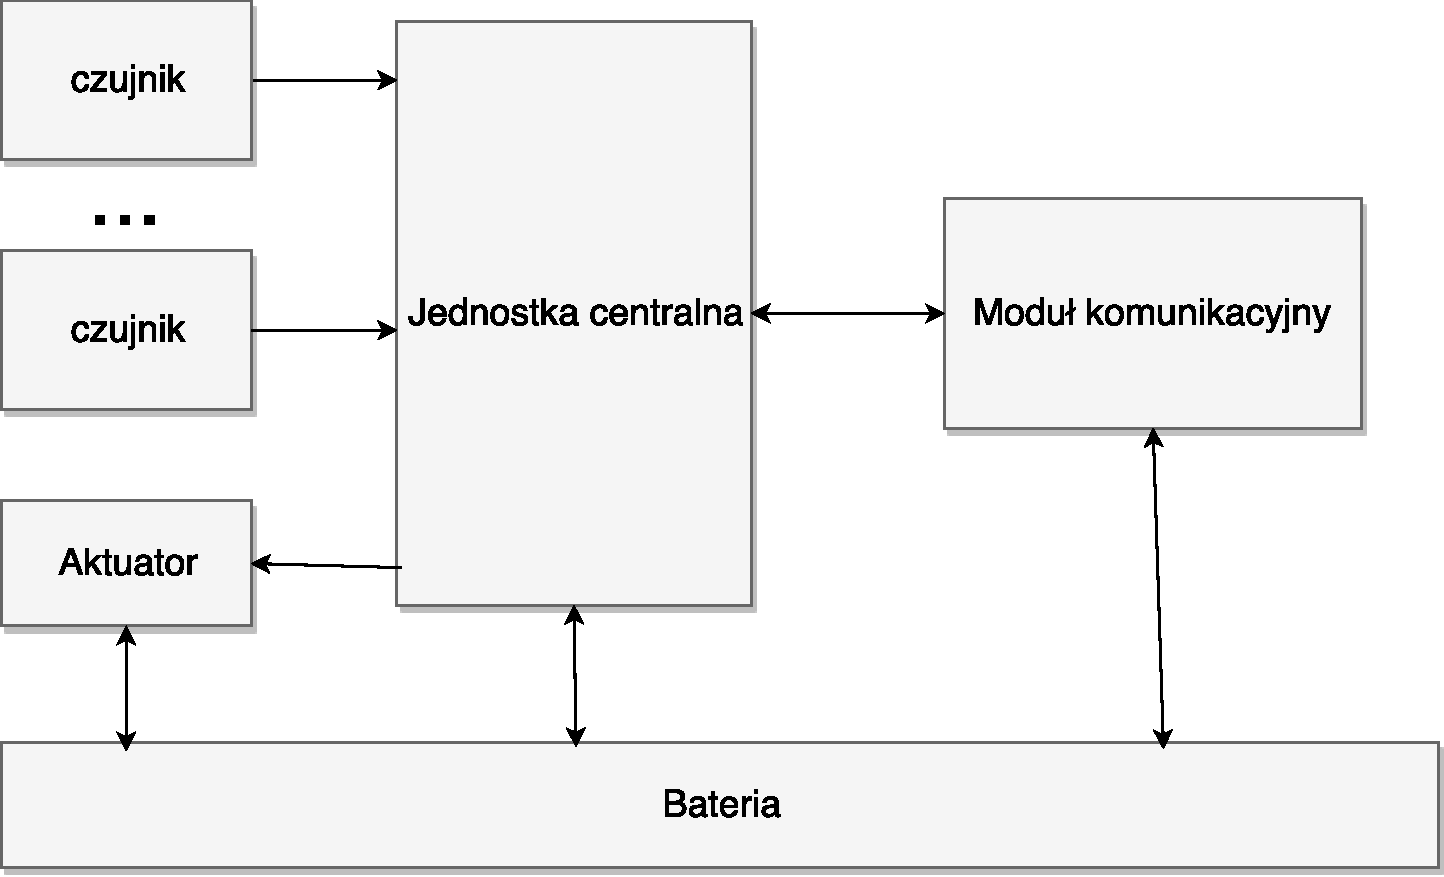
\includegraphics[scale=0.5]{\ImgPath/sensor_node.pdf}
	\end{center}
	\caption{Architektura węzła sieci czujnikowej}
\end{figure}

\section{Stos sieciowy bezprzewodowych sieci czujnikowych}

Bezprzewodowa sieć czujnikowa jest zbiorem wielofunkcyjnych węzłów czujnikowych zorganizowanych w sieć typu ad hoc. Wyróżnia się przy tym dwa główne schematy komunikacji. Pierwszym z nich odpowiada topologii gwiazdy, w której węzły komunikują się bezpośrednio z węzłem bazowym (komunikacja z jednym przeskokiem - single-hop). Drugi opisuje komunikację, w której pakiet danych przesyłany jest do węzła bazowego za pośrednictwem wielu węzłów z wykorzystaniem trasowania (komunikacja z wieloma przeskokami - multi-hop). Ten sposób pozwala na zmniejszenie zużycia energii, ponieważ zazwyczaj węzły rozmieszczone są w relatywnie małych odległościach od siebie (zagęszczenie może dochodzić nawet do 20 węzłów na $m^{3}$ \cite{Shih2001}).

Bezprzewodowe sieci czujnikowe posiadają jednak również pewne istotne różnice w stosunku do tradycyjnych sieci typu ad-hoc:
\begin{itemize}
\item Ograniczone zasoby energetyczne - często węzły sieci znajdują się w odległych, trudno dostępnych lokalizacjach, co uniemożliwia wymianę ich baterii. Wymusza to minimalizację zużycia energii, w celu uzyskania jak najdłuższego działania sieci.
\item Brak globalnych identyfikatorów węzłów sieci - w zastępstwie używana jest klasteryzacja.
\item Niedeterministyczne rozmieszczenie węzłów sieci - sieć organizuje się sama.
\end{itemize}

Stos protokołów bezprzewodowej sieci czujnikowej musi więc być zgodny z wymienionymi wcześniej cechami oraz osobliwościami tychże sieci. Okazuje się, że  stos protokołów sieciowych dla bezprzewodowych sieci czujnikowych przypomina tradycyjny model OSI (z wyłączeniem warstw prezentacji oraz sesji) \cite{Akyildiz2002.09}. Zawiera on następujące warstwy: aplikacji, transportową, sieciową, łącza danych oraz fizyczną.

\paragraph{Warstwa fizyczna}
odpowiedzialna jest za wybór częstotliwości, generowanie częstotliwości fali nośnej, wykrywanie i modulację sygnału. Przy projektowaniu warstwy fizycznej dla bezprzewodowych sieci czujnikowych zużycie energii jest istotniejszym czynnikiem od propagacji i zanikania fali. W ogólnym przypadku ilość energii potrzebna do transmisji sygnału na odległość $d$ jest proporcjonalna do $d^{n}$, gdzie $2 <= n < 4$. Wykładnik $n$ jest bliższy wartości $4$ dla nisko osadzonych w stosunku do poziomu ziemi anten \cite{Sohrabi1999} - co jest typowym przypadkiem dla sieci czujnikowych. W celu mitygacji tego problemu stosuje się komunikację wieloskokową (multi-hop) wykorzystując fakt gęstego rozmieszczenia węzłów sieci \cite{Akyildiz2002.09}.
Krytyczny dla bezawaryjnej komunikacji jest również wybór odpowiedniego rodzaju modulacji, takiego jak np. MFSK, OQPSK, MQAM czy UWB.

\paragraph{Warstwa łącza danych}
jest odpowiedzialna za multipleksowanie strumieni danych, wykrywanie ramek danych, dostęp do łącza (MAC) oraz detekcję błędów. Dla bezprzewodowych sieci czujnikowych tworzone są wyspecjalizowane protokoły MAC, które muszą spełniać dwa założenia \cite{Akyildiz2002.09, Demirkol2006}.
\begin{enumerate}
\item Stworzenie infrastruktury sieci, w tym utworzenie połączeń komunikacyjnych pomiędzy tysiącami węzłów.
\item Umożliwienie wydajnego współdzielenia zasobów komunikacyjnych pomiędzy wszystkimi węzłami sieci.
\end{enumerate}
Dodatkowo należy wziąć pod uwagę wysoką decentralizację sieci oraz jej dynamicznie zmienną topologię. Przykładami takich dedykowanych protokołów MAC mogą być S-MAC \cite{Ye2002}, WiseMAC \cite{Hoiydi2004}, CSMA \cite{Althobaiti2015} czy też TDMA \cite{Althobaiti2015}.

\paragraph{Warstwa sieciowa}
Podobnie, jak w przypadku protokołów warstwy łącza danych również i dla tej warstwy zostały stworzone dedykowane protokoły trasowania. Trasowanie w bezprzewodowych sieciach czujnikowych zostało szerzej opisane w podrozdziale \ref{routing}.

\paragraph{Warstwa transportowa}
Potrzeba wykorzystania warstwy transportowej pojawia się w momencie, gdy planowany jest dostęp do sieci czujnikowej z sieci Internet lub innej zewnętrznej sieci. Protokoły transportowe dla bezprzewodowych sieci czujnikowych powinny spełnić szereg warunków:
\begin{itemize}
\item Kontrola nad przeciążeniem sieci
\item Uproszczenie inicjowania połączeń w celu zwiększenia przepustowości sieci oraz ograniczenia opóźnień
\item Minimalizacja utraty pakietów
\item Zapewnienie każdemu węzłowi sieci takiej samej przepustowości łącza
\item Komunikacja z pozostałymi warstwami sieci - mogą one dostarczyć cennych informacji protokołowi komunikacyjnemu, np. dotyczących nieudanego trasowania.
\end{itemize}
Tradycyjnie używane protokoły takie jak TCP i UDP nie są odpowiednie dla bezprzewodowych sieci czujnikowych \cite{Fahmy2016-2}. Do dedykowanych protokołów należą m. in. CODA \cite{Wan2003}, ESRT \cite{Akan2005}, RMST \cite{Stann2003} czy PSFQ \cite{Wan2002}.

\paragraph{Warstwa aplikacji}
stanowi abstrakcję nad fizyczną topologią bezprzewodowej sieci czujników na potrzeby aplikacji. Dodatkowo zapewnia ona użytkownikom interfejs do interakcji ze światem fizycznym za pośrednictwem sieci czujników. Wyróżnia się kilka kategorii protokołów warstwy aplikacji \cite{Akyildiz2010}:
\begin{itemize}
\item Kompresja danych - stosowana jest za każdym razem, gdy dany węzeł uzyskał nową informację do przesłania. Dzięki kompresji możliwa jest minimalizacja wielkości przesyłanych pakietów danych. Najczęściej używanym rodzajem kompresji w bezprzewodowych sieciach czujnikowych jest kompresja bezstratna. Ze względu na ograniczoną pamięć oraz moc obliczeniową węzłów nie można zastosować standardowych algorytmów takich jak LZW, czy gzip. Do specjalnie zaprojektowanych na potrzeby bezprzewodowych sieci czujnikowych algorytmów należą Sensor–LZW \cite{Sadler2006} oraz DSC \cite{Slepian1973, Wyner1976}.
\item Przetwarzanie zapytań - dostęp do żądanych danych zapewnia użytkownikowi węzeł bazowy za pośrednictwem zapytań. Odpowiedzią sieci mogą być zarówno surowe dane przesłane do stacji bazowej, ale często spotykane są również bardziej wyrafinowane schematy przetwarzania zapytań uwzględniające konserwację energii. Z tego punktu widzenia, bezprzewodową sieć czujników można postrzegać jako rozproszoną bazę danych \cite{Madden2002}.
\item Zarządzanie siecią - dynamiczna natura bezprzewodowych sieci czujnikowych wymaga monitorowania oraz zarządzania jej częściami składowymi. Z potrzeby tej wynikło stworzenie dedykowanych narzędzi administracyjnych, takich jak MANNA \cite{Ruiz2003} czy SNMS \cite{Tolle2005}.
\end{itemize}

\section{Trasowanie w WSN} \label{routing}
Bezprzewodowe sieci czujnikowe mają wiele wspólnego z sieciami przewodowymi i ad-hoc, jednakże wykazują również swoje własne, unikatowe cechy oraz związane z nimi wyzwania.
Jedną z takich cech jest różnorodna gęstość sieci oraz liczby węzłów. Sieci czujnikowe mogą składać się z kilkuset do kilku tysięcy węzłów, rozmieszczonych w sposób losowy o różnorodnym zagęszczeniu. Zachowanie tych węzłów jest dynamiczne, jako że do ich zadań oprócz zbierania danych oraz przesyłania pakietów należy również oszczędzanie własnej energii. Dodatkowo duży wpływ na jakość połączenia mają wysokie poziomy szumu oraz interferencja.
Istotnym wyzwaniem związanym z sieciami czujników jest również model danych oraz ich przepływu, który różni się w zależności od konkretnego rozwiązania, w którym sieć jest wykorzystywana. Węzły sieci mogą cyklicznie wysyłać do stacji bazowej próbkę danych. W modelu zdarzeniowym węzeł sieci wysyła pakiet po wystąpieniu określonego zjawiska. Istnieją również implementacje wymagające od węzłów sieci przetwarzania oraz agregacji danych przez węzeł, przed ich wysyłką, czy takie, które wymagają komunikacji dwukierunkowej pomiędzy węzłami a stacją bazową.

%Więcej wyzwań z Routing Protocols in Wireless Sensor Networks –
%A Survey

Taka różnorodność modeli przepływu danych oraz innych wyzwań wymagają zastosowania odpowiednio zoptymalizowanych algorytmów trasowania \cite{Abdullah2014, Sohraby2006}.

Z powodu różnych potrzeb odnośnie trasowania pakietów zaproponowany został szereg metryk dotyczących zasobów sieci. Celem protokołów trasowania jest optymalizacja ich wykorzystania. \cite{Dargie2010, Biradar2009}.
\begin{itemize}
 \item Minimalizacja ścieżki pakietu do węzła bazowego
 \item Minimalizacja energii zużytej na wysłanie pakietu
 \item Maksymalizacja czasu, po którym następuje podział sieci
 \item Minimalizacja wariancji poziomów energii węzłów
\end{itemize}

\subsection{Flood}\label{subsec:flood}
Węzeł wysyłający pakiet rozgłasza go do najbliższych sąsiadów, którzy z kolei powtarzają ten krok, aż pakiet dotrze do wszystkich węzłów sieci lub osiągnie maksymalną liczbę skoków.
W przypadku tego algorytmu, jeżeli istnieje droga łącząca źródło pakietu z celem, to cel z pewnością go otrzyma.
Zaletą tego algorytmu jest jego prostota. Do wad natomiast zalicza się duży ruch pakietów w sieci. W celu jego ograniczenia oraz zapewnienia aby pakiet nie był wysyłany w nieskończoność stosowane są dwa mechanizmy \cite{Dargie2010}:
\begin{itemize}
	\item maksymalna liczba przeskoków pakietu
	\item numery sekwencji pakietów - pakiety otrzymują kolejne numery, które wraz z adresem węzła wysyłającego umożliwiają jego identyfikację. Dzięki temu węzły mogą przechowywać historię otrzymanych (oraz rozgłoszonych dalej pakietów) i w momencie w którym taki pakiet ponownie otrzymają - go odrzucić.
\end{itemize}

Mechanizmy te jednakże nie rozwiązują następujących problemów występujących w protokole Flood \cite{Dargie2010}:
\begin{itemize}
	\item Implozja - węzeł, który otrzymał pakiet rozgłasza go do swoich sąsiednich węzłów niezależnie od tego, czy otrzymały one już ten pakiet od innego węzła. Prowadzi to do niepotrzebnego zużycia zasobów. %Dorzucić obrazek
	\item Redundancję geograficzną - pakiety wysyłane przez węzły monitorujące pokrywające się obszary są traktowane jako kompletnie od siebie różne (brak fuzji danych), co prowadzi do marnowania zasobów (ta sama informacji wysyłana jest wielokrotnie). %Dorzucić obrazek
	\item Nieuwzględnianie zasobów węzła - ze względu na swoją prostotę algorytm nie bierze pod uwagę aktualnych zasobów węzła sieci, takich jak dostępna pamięć, czy energia węzła.
\end{itemize}
\subsection{SPIN}
Protokół SPIN (Sensor Protocols for Information via Negotiation) jest rodziną protokołów trasowania typu płaskiego. Do rozsyłania informacji po sieci wykorzystują one negocjację. Do ich przeprowadzenia używają pakietów zawierających metadane, które opisują przesyłane wiadomości. Dzięki temu możliwe jest wyeliminowanie redundancji transmisji występujące w protokołach typu Flood \cite{Chaudhary2015}.

Projekt SPIN wyrósł z protokołu Flood. Twórcy zauważyli trzy podstawowe problemy w tego typu podejściu, które opisane zostały w podrozdziale \ref{subsec:flood}

Innowacjami w stosunku do protokołu Flood są negocjacja oraz adaptacja w zależności od zasobów.

\paragraph{Negocjacja} W celu rozwiązania problemów związanych z implozją oraz przenikaniem się monitorowanych obszarów, przed wysłaniem pakietu węzły negocjują między sobą. Do negocjacji wykorzystywane są dodatkowe informacje o pakietach - meta-dane. 
Meta-dane wykorzystywane są do precyzyjnego opisu danych zbieranych przez czujniki. Rozmiar w bajtach meta-danych musi być mniejszy od rozmiaru samego pakietu z danymi, aby rozwiązanie miało sens.
Sam protokół nie narzuca tego co meta-dane powinny zawierać. Jest to zależne od konkretnego rozwiązania oraz implementacji. Może to być np. identyfikator węzła, współrzędne geograficzne, itd. Specyfikacja, przechowywanie oraz przetwarzanie meta-danych wykracza poza algorytm SPIN.
W protokole SPIN węzły komunikują się za pomocą trzech rodzajów pakietów:
\begin{itemize}
	\item ADV - ogłoszenie nowych danych. Jest to pakiet zawierający meta-dane. Ogłasza on węzłom pojawienie się nowych danych
	\item REQ - zgłoszenie zamówienia na dany pakiet z danymi. Węzeł, który chce otrzymać konkretny pakiet wysyła wiadomość z jego meta-danymi (tymi, które otrzymał w ADV)
	\item DATA - pakiet zawierający właściwe dane z czujnika wraz z meta-danymi
\end{itemize}
Przebieg negocjacji ilustruje rysunek \ref{fig:spin}.
\begin{figure}[H]
	\label{fig:spin}
	\begin{center}
		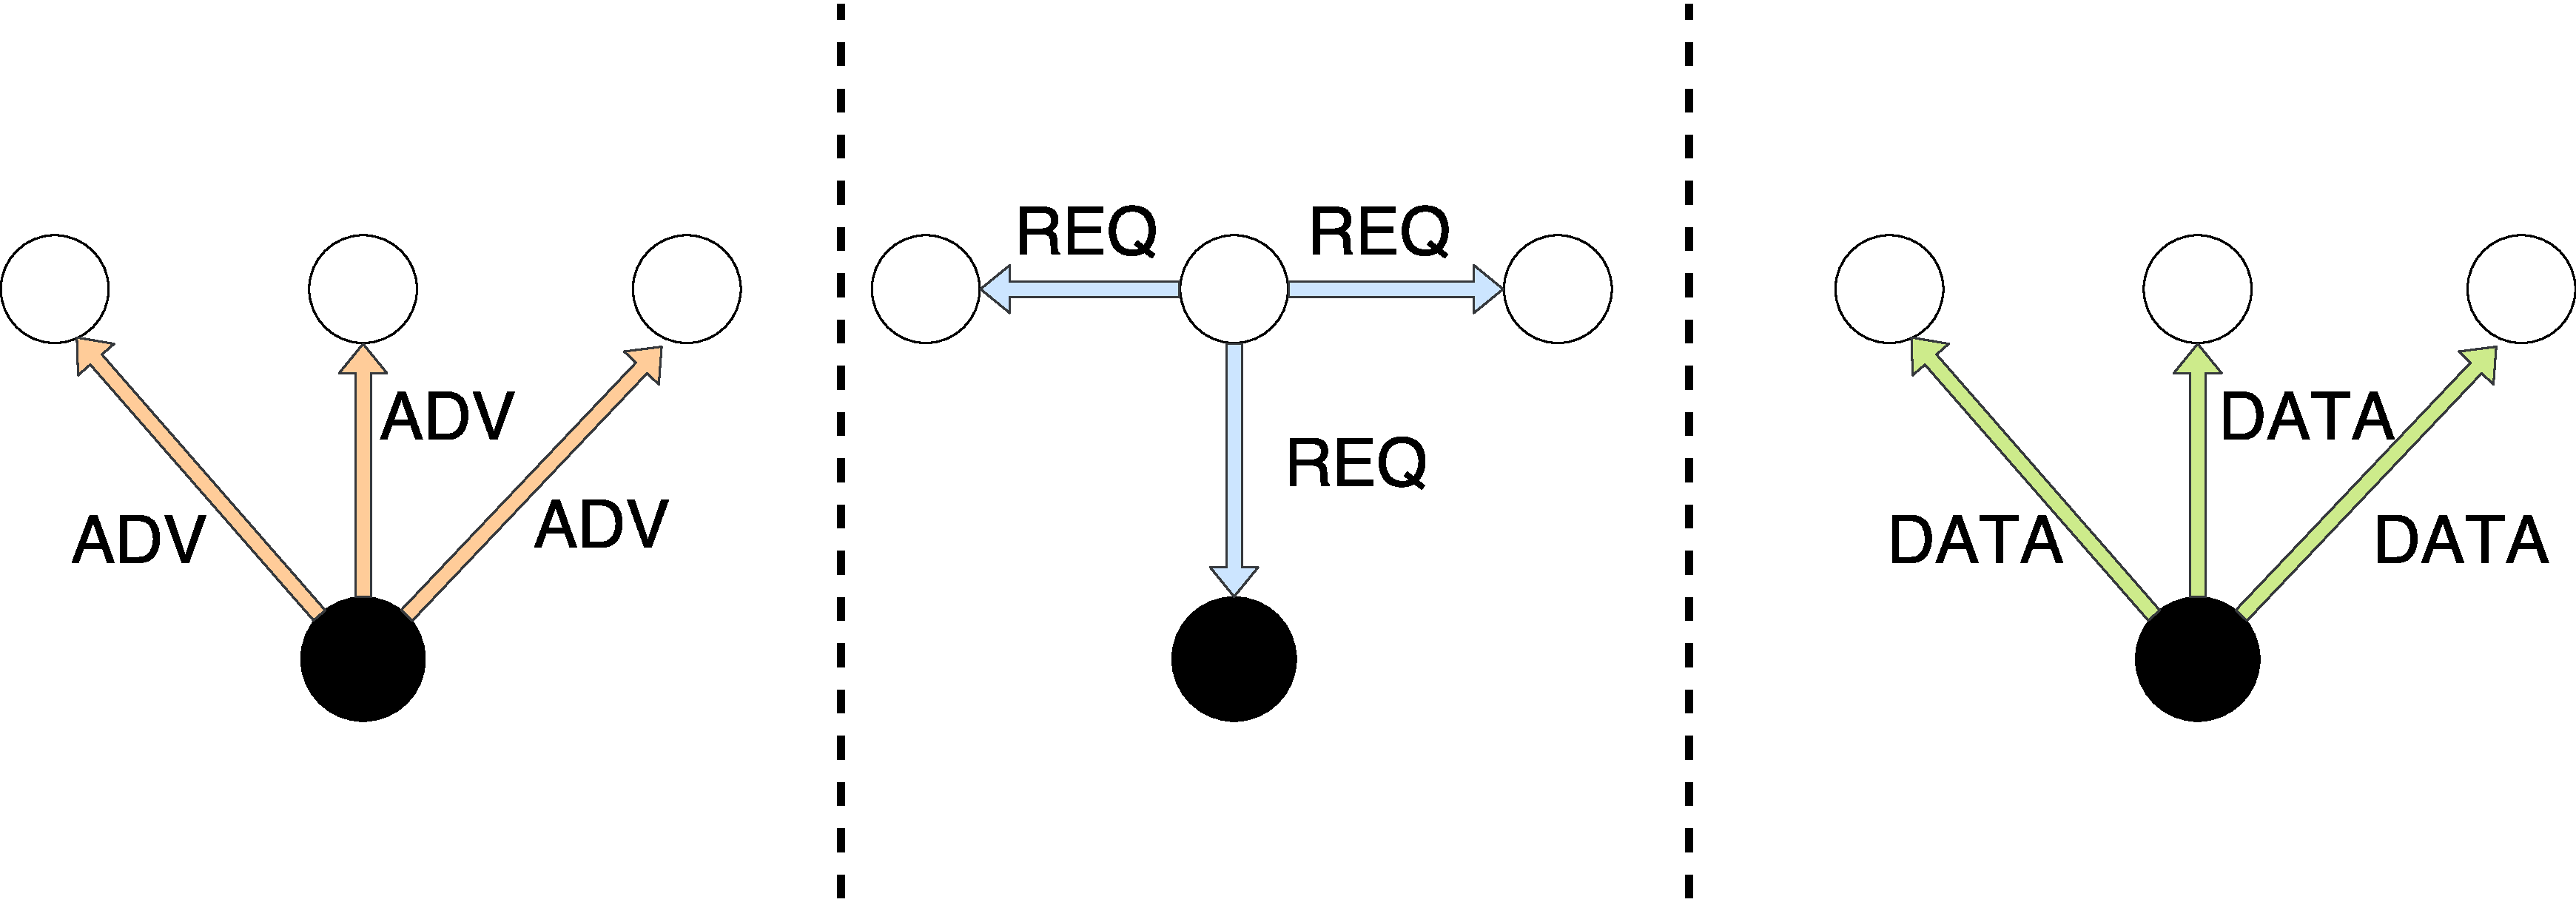
\includegraphics[scale=0.25]{\ImgPath/protocols/spin.pdf}
	\end{center}
	\caption{Przebieg negocjacji w protokole SPIN}
\end{figure}

Jako, że pakiety ADV i REQ zawierają tylko meta-dane, są one tańsze do wysłania niż DATA.

W skład rodziny algorytmów SPIN wchodzą cztery protokoły: SPIN-PP, SPIN-EC, SPIN-BC, SPIN-RL. Jako, że protokoły SPIN-PP oraz SPIN-EC nie przeznaczone są dla sieci point-to-point, opisane zostaną dwa pozostałe protokoły \cite{Dargie2010, Kulik2002}.

Protokół zaczyna się od wysłania pakietu ADV przez węzeł, który posiada nowe dane, które chce rozpropagować w sieci. Węzły sąsiednie, które otrzymały wiadomość ADV, sprawdzają czy otrzymały już takie dane. Jeśli reklamowane dane są dla nich nowe, wysyłają one wiadomość REQ z powrotem do nadawcy. Węzeł inicjujący negocjację po otrzymaniu wiadomości REQ wysyła dane w pakiecie DATA

\subparagraph{SPIN-BC}
W tym wariancie wykorzystany jest fakt, że węzły współdzielą medium komunikacyjne. Komunikacja pomiędzy dwoma węzłami może zostać ''podsłuchana'' przez węzły znajdujące się w zasięgu. Wszystkie pakiety wysyłane są w trybie rozgłoszeniowym, jako że dla sieci bezprzewodowej nie wiąże się to z dodatkowym kosztem.

Wiadomość ADV jest rozgłaszana do wszystkich sąsiednich węzłów. Jednakże przed wysłaniem wiadomości REQ węzły czekają przez losowy okres. Jeżeli węzeł przechwycił wiadmość REQ dotyczącą tych samych danych, których i on potrzebuje, anuluje on wysyłkę swojej wiadomości REQ (nie jest potrzebna, redukuje to koszty). Pozwala to również na uniknięcie kolizji. Po otrzymaniu REQ węzeł wysyła pakiet DATA do kanału rozgłoszeniowego. Pakiet DATA jet wysyłany tylko raz, następujące po nim wiadomości REQ dotyczące tych samych danych są ignorowane.
\subparagraph{SPIN-RL}
SPIN-RL jest przystosowaniem SPIN-BC do warunków komunikacji stratnej. Każdy węzeł przechowuje listę wiadomości ADV i jeśli nie otrzyma on danych w odpowiednim czasie, to ponawia on wysyłkę zapytania o dane (REQ). Odbiorca jest losowany z listy węzłów które wysłały ogłoszenie o tych samych danych.
Po wysyłce pakietu DATA musi upłynąć pewien odstęp czasowy przed ponowną wysyłką.

%Zakończenie
Zgodnie z badaniami opisanymi w artykule \cite{Kulik2002} protokoły SPIN są w stanie dostarczyć 60\% więcej danych w sieciach point-to-point i 80\% więcej danych w sieciach rozgłoszeniowych niż tradycyjne rozwiązania.  
\subsection{LEACH} \label{subsec:leach}
LEACH jest protokołem typu hierarchicznego, który wykorzystuje dwa poziomy grupowania węzłów. Pakiety trasowane są od czujników do lokalnych węzłów bazowych i od lokalnych węzłów bazowych do stacji bazowej \cite{Yu2006}.
Węzły same organizują się w klastry, w których jeden węzeł pełni funkcję lokalnego węzła bazowego - nazywany jest on również Cluster Head. W przeciwieństwie do konwencjonalnych algorytmów lokalne węzły bazowe nie są wybierane a priori. Wybierane są rotacyjnie w sposób losowy, tak aby równomiernie rozłożyć zużycie energii oraz wybierać węzły z możliwie jak największą energią. Dodatkowo LEACH wykorzystuje fuzję danych w celu skompresowania ich ilości przesyłanych z klastra do stacji bazowej \cite{Akkaya2005, Heinzelman00}.

Działanie algorytmu podzielone jest na rundy. Każda runda składa się z fazy konfiguracyjnej, po której następuje faza stabilnego działania sieci. W fazie początkowej każdy węzeł decyduje o tym czy ma zostać lokalnym węzłem bazowym w aktualnej rundzie. Decyzja ta opiera się na zadanej przez użytkownika liczbie lokalnych węzłów bazowych w sieci (wyrażonej jako procent liczby wszystkich węzłów sieci) oraz na fakcie uprzedniego bycia lokalnym węzłem bazowym.
Algorytm ten przebiega w sposób następujący:
\begin{enumerate}
	\item Węzeł n losuje liczbę z zakresu od 0 do 1
	\item Obliczany jest próg wyrażony poniższym wzorem
	\[T(n) = \begin{dcases} 
      \frac{P}{1-P*(r\:mod\frac{1}{P})} & n \in G \\
      0 & n \not\in G \\
   \end{dcases}
	\]
	, gdzie P - procent sieci, którą powinny stanowić lokalne węzły bazowe,
	r - numer aktualnej rundy
	G - zbiór węzłów, które nie były lokalnymi węzłami bazowymi przez ostatnie $\frac{1}{P}$ rund.
	\item Jeżeli wylosowana liczba jest mniejsza od progu $T(n)$, to węzeł zostaje lokalnym węzłem bazowym.
\end{enumerate}
Taki wybór lokalnych węzłów bazowych gwarantuje, że każdy węzeł sieci zostanie nim w ciągu $\frac{1}{P}$ rund. Wszystkie węzły, które zostały wybrane jako lokalne węzły bazowe w pierwszej rundzie (o numerze 0) nie zostaną nimi przez kolejnych $\frac{1}{P}$ rund. Przez kolejne rundy wartość progu $T(n)$ rośnie. Funkcja została zaprojektowana w ten sposób, aby wraz ze zmniejszaniem się liczby węzłów, które mogą zostać potencjalnie wybrane na lokalne węzły bazowe prawdopodobieństwo ich wyboru rosło. Po $\frac{1}{P}$ rundach próg $T(n)$ wraca do stanu początkowego, tym samym rozpoczynając ponownie opisany cykl.
Powyższy algorytm zakłada, że wszystkie węzły są homogeniczne pod względem początkowej ilości energii oraz jej zużywania.

Węzeł, który został wybrany na lokalny węzeł bazowy ogłasza ten fakt  pozostałym węzłom. Wykorzystywany jest przy tym protokół MAC CSMA. W tym czasie pozostałe węzły sieci muszą mieć włączone odbiorniki radiowe. Po zakończeniu tej fazy każdy z węzłów sieci nie będący lokalnym węzłem bazowym dokonuje decyzji, do którego klastra będzie należeć. Wybrany zostaje ten klaster, od którego zostało otrzymane ogłoszenie o największym wskaźniku mocy odebranego sygnału (z ang. RSSI - Received Signal Strength Indication). Dzięki tymi wybrany zostaje lokalny węzeł bazowy, z którym komunikacja jest najmniej kosztowna energetycznie.

Po dokonaniu wyborów klastrów przez węzły muszą one ów wybór zakomunikować lokalnym węzłom bazowym. Wysyłają więc one pakiet informujący o dołączeniu do klastra lokalnym węzłom bazowym (również z wykorzystaniem protokoły MAC CSMA).

Po otrzymaniu informacji zwrotnej od węzłów, lokalne węzły bazowe tworzą harmonogramy TDMA na podstawie liczby węzłów w klastrze. Wykorzystanie TDMA umożliwia zredukowanie kolizji podczas komunikacji \cite{Ilyas2004, Ergen2010}. Z pozostałego czasu rundy przeznaczonego na fazę stabilną wydzielane są dla każdego węzła przedziały czasowe, podczas których mogą one wysłać swoje pakiety z danymi do lokalnego węzła bazowego \cite{Cionca2008}. Harmonogram zostaje rozgłoszony do wszystkich węzłów w klastrze.

Po utworzeniu klastrów oraz harmonogramów TDMA, następuje faza stabilnego działania sieci, podczas której węzły przesyłają zebrane dane do lokalnych węzłów bazowych. Każdy węzeł transmituje pakiety w wyznaczonym dla niego przedziale czasowym. Transmisja odbywa się przy użyciu minimalnej energii, tak aby pakiet mógł dotrzeć do lokalnego węzła bazowego. Pozostałe węzły w klastrze (nie biorące udziału w transmisji) mogą w tym czasie wyłączyć odbiorniki radiowe w celu oszczędzania energii. Po otrzymaniu pakietu z danymi, lokalny węzeł bazowy przetwarza go oraz agreguje zgodnie z zaimplementowanymi regułami. Sposób kompresji oraz agregacji sygnałów jest dostosowywany do specyfiki danych zbieranych przez sieć (np. dane o temperaturze mogą zostać uśrednione w pewnym przedziale czasu). Po zebraniu danych lokalny węzeł bazowy przesyła je w pakiecie do stacji bazowej, po czym następuje nowa runda \cite{Yadav2014}.
\begin{figure}[H]
	\begin{center}
		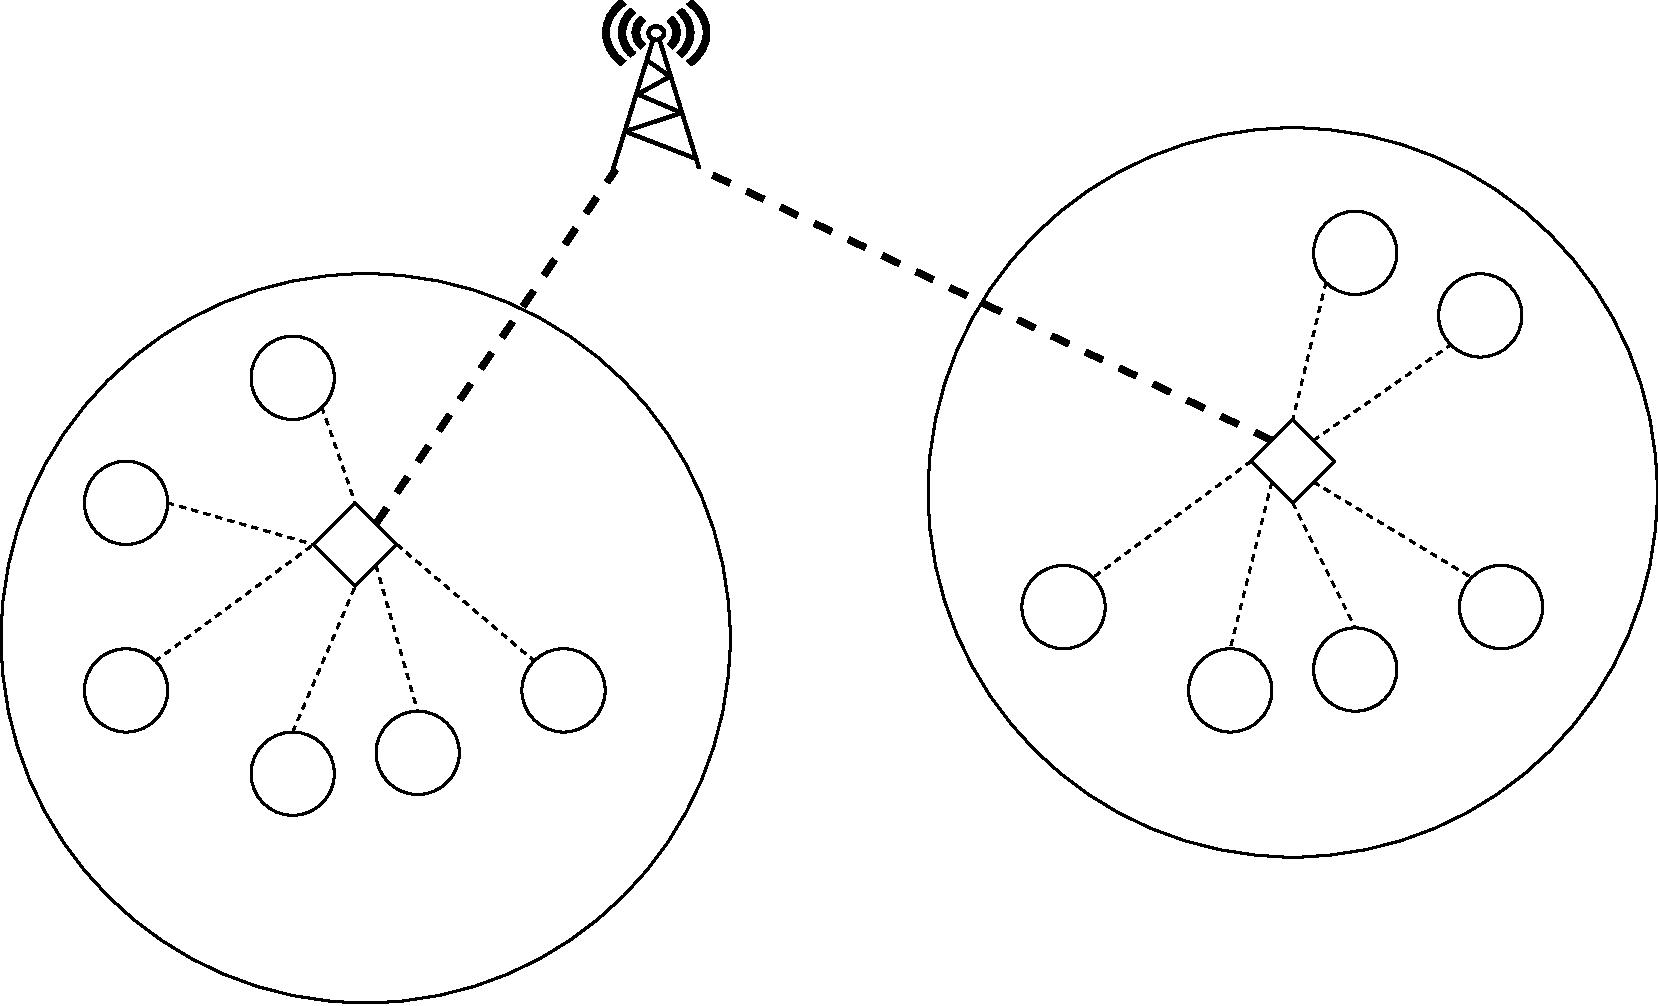
\includegraphics[scale=0.3]{\ImgPath/protocols/leach.pdf}
	\end{center}
	\caption{LEACH}
\end{figure}
\paragraph{ALEACH (Advanced LEACH)} \label{para:aleach}
ALEACH zmienia sposób wyboru lokalnego węzła bazowego. Nowy sposób obliczania progu $T(n)$ opiera się na nowych parametrach nazwanych prawdopodobieństwem aktualnego stanu oraz globalnym prawdopodobieństwie \cite{Ali2008}.

\[
	T(n) = G_{p} + CS_{p}
\]

Prawdopodobieństwo aktualnego stanu ($CS_{p}$) wyrażone jest poniższym wzorem \cite{Ali2008}.
\[
	CS_{p} = \frac{E_{aktualne}}{E_{n-max}}*\frac{K}{N}
\]
Gdzie $E_{aktualne}$ oznacza aktualną energię węzła, $E_{n-max}$ stanowi początkową energię sieci, $K$ spodziewaną liczbę lokalnych węzłów bazowych w rundzie, a $N$ liczbę wszystkich węzłów sieci. Im większa energia pozostała w danym węźle, tym większe jest prawdopodobieństwo, że zostanie on lokalnym węzłem bazowym.

Prawdopodobieństwo globalne natomiast liczone jest zgodnie ze wzorem \cite{Ali2008}:
\[
	G_{p} = \frac{K}{N - K * (r \:mod \frac{N}{K})}
\]

Pozostała część algorytmu jest taka sama jak w LEACH. Dzięki uwzględnieniu podczas wyboru lokalnego węzła bazowego jego aktualnej energii algorytm ten pozwala na wydłużenie życia sieci w stosunku do LEACH \cite{Singh2017}.
\paragraph{LEACH DCHS (LEACH-Deterministic Cluster Head Selection)}
Celem tego wariantu protokołu LEACH, tak samo jak w przypadku ALEACH, jest wydłużenie działania sieci czujników. Efekt ten został uzyskany dzięki modyfikacji progu $T(n)$ \cite{Handy2002, Singh2017}.
 \[
	T(n) =  \frac{P}{1 - P * (r \:mod \frac{1}{P})} * \left[\frac{E_{n_{aktualne}}}{E_{max}} + \left(r_{s} \backslash \frac{1}{p}\right)\left(1 - \frac{E_{n_{aktualne}}}{E_{max}}\right)\right]
\]

Włączenie aktualnego poziomu energii węzła do wzoru umożliwia zwiększenie prawdopodobieństwa wyboru węzła o większej energii na lokalny węzeł bazowy. Dodatkowo wraz z upływem czasu zwiększa się prawdopodobieństwo wyboru węzłów, które najdłużej nie pełniły tej funkcji. Odpowiada za to fragment $r_{s} \backlash \frac{1}{p}$.

\chapter{Narzędzia do symulacji sieci}
% Wykorzystany symulator zdarzeń dyskretnych, opisać po krótce inne
% 1-2 strony
Rozdział ten opisuje narzędzia oraz technologie, które zostały użyte do symulacji działania sieci czujników, implementacji protokołów trasowania oraz przeprowadzenia testów.
\section{Przegląd narzędzi}
\cite{Xian2008}
\cite{Nayyar2015}
\subsection{NS-2}
\subsection{NS-3}
\subsection{IKR}
\subsection{openWNS}
\subsection{Matlab}
\subsection{OPNET}
\subsection{J-Sim}
\subsection{SensorSim}
\subsection{NCTUns}
\subsection{SSFNet}
\subsection{QualNet}
\subsection{SENSE}
\section{\omnetpp}
\omnetpp jest zbudowanym w sposób modularny symulatorem zdarzeń dyskretnych. Stanowi on ogólne narzędzie umożliwiające przeprowadzanie symulacji między innymi: przewodowych oraz bezprzewodowych sieci komputerowych, systemów wieloprocesorowych, chmur obliczeniowych czy też ruchu miejskiego. Dla każdej bardziej wyspecjalizowanej dziedziny konieczne jest stworzenie nowego modelu (zbioru modułów) lub skorzystanie z jednego z już istniejących rozwiązań (np. INET, VEINS).\cite{Varga2017}
\subsection{Moduły}
Podstawowym budulcem symulacji w \omnetpp są moduły. Dzielą się one na proste oraz złożone.
% Opis co to moduł oraz że są proste i złożone, możne je zagneżdżać oraz wiązać za pomocą bram (ang. gate). A komunikują się za pomocą wiadomości i sygnałów

Do implementacji modułów wykorzystuje się dwa języki
\begin{enumerate}
	\item NED - język domenowy \omnetpp, za pomocą którego definiowane są moduły. Zawierają opis parametrów oraz bram modułu. Dodatkowo w przypadku modułów złożonych definiowane są zagnieżdżone moduły wraz z ich połączeniami.
	%Wstawić przykład
	\item C++ - wykorzystywany do implementacji modułów prostych (moduły złożone definiowane są tylko za pomocą plików NED).
	%Wstawić przykład
\end{enumerate}
Dodatkowo, w celu przyspieszenia oraz ułatwienia implementacji wiadomości, które moduły wykorzystują w komunikacji stworzono odpowiedni język dziedzinowy, który tłumaczony jest przez kompilator do kodu C++.
%Wstawić przykład

Moduły umieszczane są w Sieciach (Network), które również zdefiniowane są w języku NED.

Do komunikacji moduły wykorzystują zdefiniowane (w pliku .ned) przez programistę łącza (ang. links ) oraz bramy (ang. gates).
\subsection{Przeprowadzenie symulacji}
\omnetpp umożliwia skorzystanie z różnych interfejsów użytkownika: QT, TKenv oraz wiersza poleceń. W fazie testowania poprawności przygotowanej symulacji skorzystać można z jednego z interfejsów graficznych. Po weryfikacji zalecana jest rezygnacja z interfejsu graficznego w celu przyspieszenia działania symulacji. Niebywałym ułatwieniem w przygotowaniu oraz uruchomieniu zestawu symulacji w celu zebrania danych do analizy są pliki konfiguracyjne. Umożliwiają one określenie parametrów modułów wchodzących w skład sieci oraz zadeklarowanie parametrów wchodzących w skład zmiennych badanych w ramach symulacji (parameter studies).
%Wstawić przykład
\section{INET}
INET jest biblioteką/modelem zawierającym implementacji wielu protokołów sieciowych (m.in. IPv4, IPv6, TCP, SCTP, UDP), jak również standardów komunikacji wykorzystywanych m.in. w sieciach czujników (IEEE 802.15.4).\cite{inet}

%Opisać, że biblioteka zawierała błędy, opisać jakie błędy i jak zostały naprawione

\chapter{Implementacja}
W ramach pracy powstała minibiblioteka zawierająca moduły ułatwiające implementację protokołów działających w ramach WSN. Stanowi ona rozszerzenie biblioteki INET, zawierającej moduły dla standardu IEEE 802.15.4.

Biblioteka składa się z następujących modułów:
\begin{itemize}
	\item WSNNode --- złożony moduł ,,abstrakcyjny'' stanowiący bazę dla węzłów sieci. W jego skład wchodzą:
\paragraph{Moduł mobilności} Jest to moduł zarządzający położeniem oraz mobilnością węzła. Jako, że zakres pracy obejmuje węzły stacjonarne, jako wartość domyślna został przyjęty moduł StationaryMobility, który jedynie śledzi położenie węzła.
\paragraph{Źródło energii} Jako źródło energii wykorzystany został udostępniony przez Inet moduł prostego zasobnika energii (SimpleEnergyStorage).
\paragraph{Tablica interfejsów} Przechowuje informacje o interfejsach danego węzła. W przypadku objątych tą pracą symulacji jest to jeden interfejs radiowy.
\paragraph{Moduł stanu węzła} Jest to moduł informujący o aktualnym stanie węzła.
\paragraph{Moduł monitora} Jest to autorski moduł monitorujący poziom energii w węźle do celów statystycznych. Moduł w regularnych odstępach czasu emituje sygnał zawierający aktualną ilość energii w węźle.
\paragraph{Moduł warstwy sieciowej} Odpowiada za warstwę sieciową węzła. Zawierają się w nim moduły odpowiedzialne za trasowanie pakietów.
\paragraph{Moduł karty sieciowej} Jest to moduł symulujący kartę sieciową. Zawiera się w nim moduł odpowiadający za warstwę fizyczną oraz moduł łącza danych.
\begin{figure}[!htbp]
	\begin{center}
		\centering
		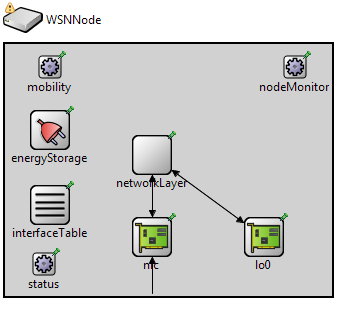
\includegraphics[scale=1]{\ImgPath/framework/node.png} 
	\end{center}
	\caption{Węzeł sieci}
	\label{abstractNode}
\end{figure}
\FloatBarrier
	\item WSNSensorNode - dziedziczy po WSNNode oraz zawiera dodatkowo moduł generujący pakiety
	\begin{figure}[!htbp]
	\begin{center}
		\centering
		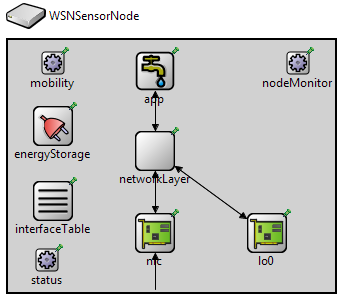
\includegraphics[scale=1]{\ImgPath/framework/sensor.png} 
	\end{center}
	\caption{Czujnik}
	\label{openlayers}
\end{figure}
\FloatBarrier
	\item WSNSinkNode - dziedziczy po WSNNode oraz zawiera dodatkowo moduł akcetujący pakiety od czujników
	\begin{figure}[!htbp]
	\begin{center}
		\centering
		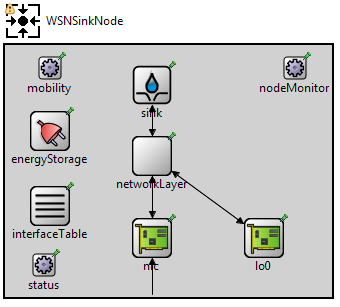
\includegraphics[scale=1]{\ImgPath/framework/sink.png} 
	\end{center}
	\caption{Stacja bazowa}
	\label{abstractNode}
\end{figure}
\FloatBarrier
	\item NodeCounter - moduł liczący działające węzły w sieci
	\item SimpleEnergyConsumer - moduł pobierający energię na żądanie
	\item VolatileStateBasedEnergyConsumer - moduł pobierający energię w zależności od ustawionego stanu z możliwością dynamicznej zmiany poboru mocy
\end{itemize}
\section{Protokoły}
Każda implementacja wybranego algorytmu trasowania wymaga stworzenia dwóch modułów. Jeden z nich dziedziczy po SimpleNetworkLayer, a drugi po NetworkProtocolBase.

Głównymi funkcjami, które jednocześnie wywoływane są przez silnik symulacji są handleSelfMessage, handleUpperPacket oraz handleLowerPacket.

\begin{minted}{cpp}
    virtual void handleSelfMessage(cMessage *msg) override;

    virtual void handleUpperPacket(cPacket *) override;

    virtual void handleLowerPacket(cPacket *) override;
\end{minted}
% flood jako akapit
\subsection{Flood}
W implementacji protokołu Flood wykorzystany został istniejący już moduł z biblioteki INET. Należało jedynie utworzyć  moduł będący warstwą sieciową, a następnie skonfigurować go, aby wykorzystywał moduł Flood z biblioteki INET.
\subsection{SPIN}
Protokół SPIN został zaimplementowany zgodnie z zaproponowanym w artykule \cite{Kulik2002} wariancie SPIN-RL.

Kod odpowiadający za logikę protokołu znajduje się w klasie SPIN, która dziedziczy po klasie NetworkProtocolBase oraz implementuje interfejs INetworkProtocol z biblioteki INET.

\begin{minted}{cpp}
class SPIN : public NetworkProtocolBase, public INetworkProtocol
\end{minted}

Moduł po otrzymaniu pakietu z wyższej warstwy dokonuje decyzji, czy węzeł ma dostatecznie dużo energii, aby przeprowadzić negocjację. W przypadku pozytywnej decyzji rozpoczynany jest proces negocjacji. W przeciwnym wypadku dane rozgłaszane są bezpośrednio, z pominięciem negocjacji. Obrazuje to poniższy fragment kodu.

\begin{minted}{cpp}
void SPIN::handleUpperPacket(cPacket *m)
{
    SPINDatagram *msg = encapsMsg(m, DATA);
    msg->setSeqNum(seqNum);
    seqNum++;

    if (isNegotiationViable()) {
        advertiseData(msg);
    } else {
        simpleSend(msg);
    }
    nbDataPacketsSent++;
}
\end{minted}

Teoretyczny opis protokołu SPIN nie zawiera algorytmu, który węzły powinny wykorzystywać przy podejmowaniu decyzji czy rozpoczęcie procesu negocjacji jest zasadne z punktu widzenia konserwacji zasobów energetycznych. W implementacji zaproponowany więc został algorytm wykorzystujący funkcję wygładzającą o poniższym wzorze ogólnym:
\[
	f(x) = \frac{k*x}{k - x + 1}
\]

Jako parametr k przyjęte zostało 1,2, a jako zmienną x stosunek aktualnej energii węzła do jego energii maksymalnej. Po podstawieniu otrzymuje się poniższy wzór, który został wykorzystany bezpośrednio w implementacji: 

\[
	f(E_{akt}, E_{max}) = \frac{1.2 * \frac{E_{akt}}{E_{max}}}{1.2 - \frac{E_{akt}}{E_{max}} + 1}
\]
Algorytm decyzyjny przedstawiony jest na poniższym listingu. Z przedziału [0, 1] losowana jest liczba, która następnie porównywana jest z wartością wcześniej opisanej funkcji. Jeżeli wylosowana liczba jest od niej mniejsza, podejmowana jest pozytywna decyzja o podjęciu negocjacji.
\begin{minted}{cpp}
bool SPIN::isNegotiationViable()
{
    double randomNumber = uniform(0, 1);
    double k = -1.2;
    double currentEnergyFrac = currentEnergy / maxEnergy;

    return randomNumber < (k*currentEnergyFrac / (k -
        currentEnergyFrac + 1));
}
\end{minted}
\subsection{LEACH}
Implementacja protokołu LEACH została wykonana na bazie implementacji z symulatora Castalia.
\subsection{ALEACH}
W ALEACH zmieniony został sposób wyboru lokalnego węzła bazowego. W implementacji wykorzystany został mechanizm dziedziczenia. Klasa ALEACH stanowi rozszerzenie wcześniej zaimplementowanej klasy LEACH. Jedyną zmianą jest przesłonięcie funkcji selectCH za pomocą tej zdefiniowanej na listingu poniżej, która realizuje założenia zawarte w akapicie \nameref{para:aleach} zawartym w sekcji \ref{subsec:leach}.
\begin{minted}{cpp}
void ALEACH::selectCH()
{
    ...
    double generalProb = (double)expectedCHNum / 
        (double)(numSensors - expectedCHNum * 
            (roundNumber % (numSensors / expectedCHNum) ));
    double currentEnergy = 
        energyStorage->getResidualCapacity().get();
    double currentStateProb = (currentEnergy / maxEnergy) *
        ((double) expectedCHNum / numSensors);
    ...
}
\end{minted}
\subsection{LEACH DCHS}
Protokół Leach DCHS zaimplementowany został w sposób analogiczny do protokołu ALEACH.
\begin{minted}{cpp}
void LEACH_DCHS::selectCH()
{
   ...
   probability = percentage / (1 - percentage * (roundNumber
       % (int)(1/percentage)))
       * (currentEnergy / maxEnergy +
       (notCHRounds / (1/percentage))
       * (1 - (currentEnergy / maxEnergy)));
   ...
}
\end{minted}
\section{Poprawa biblioteki INET}
Umożliwienie warstwie sieciowej dostępu do rssi. Problem został już wcześniej zasygnalizowany przez jednego z użytkowników, jednakże nie został on rozwiązany. Znajomość rssi jest niezbędna do prawidłowego działania algorytmów opartych na LEACH.

Dodanie możliwości zmiany modułu MAC w Ieee802154NarrowbandNic.

Poprawa modułu IPvXTrafGen, tak aby prawidłowo zachowywał się podczas deaktywacji węzła.

Uzupełnienie modułu CSMA o funkcje obsługujące jego wyłączenie oraz ponowne włączenie. Przed poprawką, wyłącznie się symulowanego węzła (w wyniku zużycia energii) powodowało wystąpienie wyjątku i awaryjne zakończenie symulacji.

Obsługę przypadku, gdy pakiet dociera do wyłączonego już węzła.

Przeniesienie trzech poprawek autorstwa Floriana Kauera dotyczących szczegółów związanych z danymi zaczerpniętymi ze specyfikacji mikrokontrolera na podstawie której zdefiniowano domyślne parametry w Inecie.

\chapter{Symulacje}
W ramach pracy został przeprowadzony zestaw scenariuszy symulacyjnych. Każdy z zaimplementowanych protokołów został przetestowany z przygotowanymi zestawami parametrów wejściowych.
Do tych parametrów należą:
\paragraph{Dystrybucja węzłów sieci}
Symulacje zostały przeprowadzone dla dwóch sposobów dystrybucji węzłów: zgodnej z rozkładem normalnym oraz zgodnej z rozkładem jednorodnym.

Dla rozkładu normalnego średnia współrzędnej wynosiła 400m, a jej odchylenie standardowe 100m.

\begin{figure}[!htbp]
	\begin{center}
		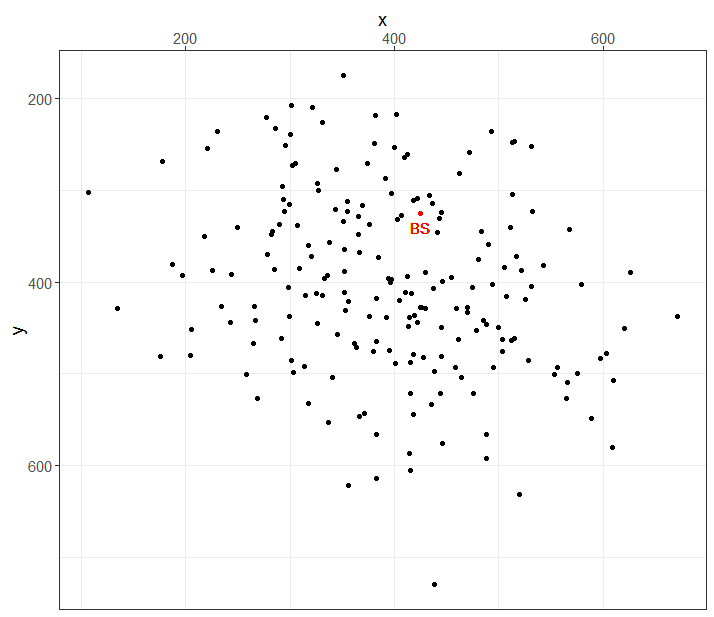
\includegraphics[scale=0.75]{\ImgPath/charts/normal_distribution.png}
	\end{center}
	\caption{Przykładowa dystrybucja węzłów sieci zgodna z rozkładem normalnym}
\end{figure}

Z rozkładem jednorodnym węzły zostały rozłożone na obszarze o kształcie prostokąta o wymiarach 450m na 550m.

\begin{figure}[!htbp]
	\begin{center}
		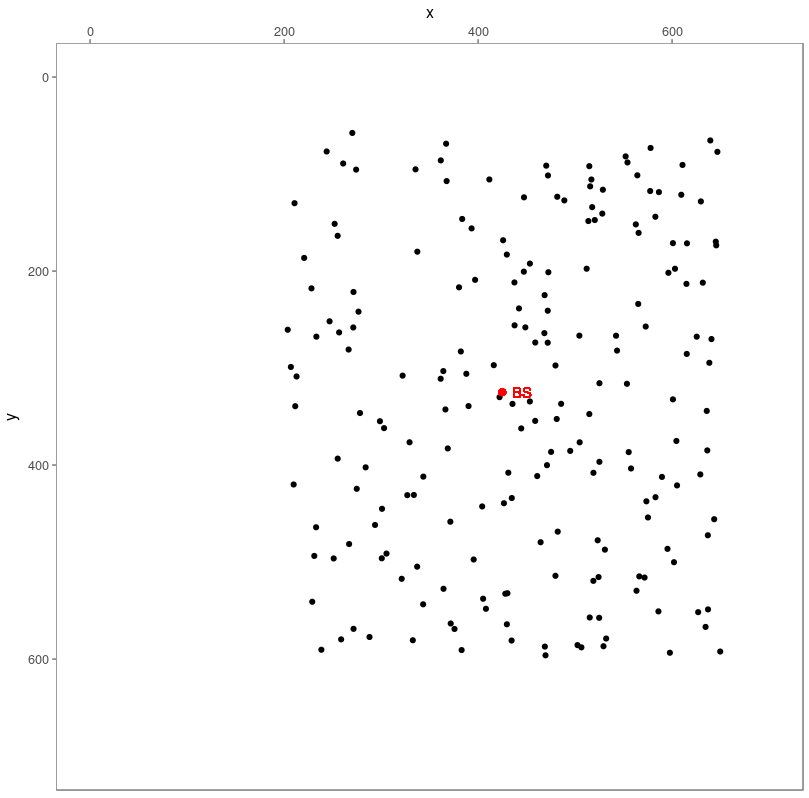
\includegraphics[scale=0.75]{\ImgPath/charts/uniform_distribution.png}
	\end{center}
	\caption{Przykładowa dystrybucja węzłów sieci zgodna z rozkładem jednorodnym}
\end{figure}

\paragraph{Liczba węzłów sieci}
Symulacje przeprowadzono dla sieci składającej się z dwudziestu oraz dwustu czujników.
\paragraph{Rozmiar pakietu z danymi}
Symulacje przeprowadzono dla rozmiarów pakietów 5B, 50B, 500B, 5000B.
\paragraph{Częstotliwość generowania nowych danych}
Symulacje przeprowadzono dla okresów generowania danych wynoszących: 5s, 10s, 15s, 20s.
\paragraph{Początkowa wartość energii elektrycznej w węźle}
Jako początkową wartość dla czujnika przyjęto 5J, co odpowiada baterii R6 (AA) w skali 1:1000.
%uzasadnić na krzywej zużycia baterii

Dodatkowo dla protokołów z rodziny LEACH zdefiniowane zostały parametry:
\paragraph{Procent lokalnych węzłów bazowych w sieci}
\paragraph{Długość rundy}

W celu zniwelowania wpływu losowego rozmieszczenia węzłów na długość działania sieci, dla każdego pojedynczego zestawu parametrów wykonano 5 przebiegów symulacji z różnym ziarnem. Wyniki tych przebiegów zostały uśrednione.

Dla każdej symulacji zostały również zdefiniowane stałe warunki środowiskowe:
\begin{itemize}
	\item Przestrzeń - idealnie płaski teren bez żadnych przeszkód.
	\item Prędkość propagacji fali - założono model propagacji fali ze stałą prędkością. Oznacza to, że czas propagacji jest proporcjonalny do przebytej odległości zdeterminowanej przez stały parametr prędkości.
	\item Tłumienie trasy radiowej - założono model Breakpoint path loss.
	\item Szum tła - założono szum izotropowy o mocy -96.616dBm.
	\item Do reprezentacji sygnału analogowego wykorzystany został model skalarny - opisuje on sygnał za pomocą jego mocy skalarnej, szerokości pasma oraz częstotliwości fali nośnej.
\end{itemize}

\section{Analiza danych}
\subsection{Aktywne czujniki}
Ogólna tendencja - im większy rozmiar pakietu oraz krótszy odstęp, tym  szybsze tempo wyłączania się węzłów sieci.

Algorytmy Flood oraz SPIN wykazują jednakowe tempo spadku liczby aktywnych czujników, niezależne od rozmiaru pakietu oraz okresu między pakietami. W przypadku również większość czujników wyłącza się w bardzo krótkim przedziale czasowym. Oznacza to, że zużycie energii przez węzły jest równomierne (wszystkie czujniki są przez cały czas swojej aktywności w trybie nasłuchiwania - w przeciwieństwie do rodziny alogrytmów typu LEACH, w których występują okresy ''uśpienia'' czujników).

Sieci korzystające z protokołów LEACH, ALEACH i LEACH DCHS wykazują wyraźnie dłuższe działanie niż sieci używające Flood i SPIN.
Różnice zacierają się dla większych rozmiarów pakietów i mniejszych odstępów czasu pomiędzy pakietami.

Różnice pomiędzy grupami protokołów są wyraźniejsze dla sieci z liczbą węzłów 200.

Poniższe wykresy przedstawiają liczbę aktywnych węzłów sieci w czasie oraz w zależności od rozmiaru pakietu i odstępie czasu pomiędzy kolejnymi pakietami. Sieć składała się z dwudziestu węzłów, które rozmieszczone zostały zgodnie z rozkładem normalnym.
Przy rozmiarach pakietu wynoszących 50B i 500B najdłuższy czas działania sieci osiągnięto wykorzystując protokół ALEACH. Czas działania sieci używających wariantów protokołu LEACH uległ wyraźnemu skróceniu przy rozmiarze pakietu wynoszącym 5000B. Wpływ okres pomiędzy pakietami na protokoły typu LEACH jest również zauważalny, jednakże jest on zdecydowanie mniej wyrazisty. Czas działania sieci dla protokołów Flood i SPIN pozostaje niezmienny, niezależnie od dobranych parametów wykresu. Dodatkowo w ich przypadku deaktywacja węzłów sieci przebiega gwałtownie oraz lawinowo - większość węzłów sieci zostaje wyłączonych w okolicach jednego punktu w czasie.

Przy rozmiarze pakietu 5B najlepszymi protokołami z punktu widzenia całkowitej długości życia sieci okazały się ALEACH oraz LEACH DCHS.

\begin{figure}[H]
	\begin{center}
		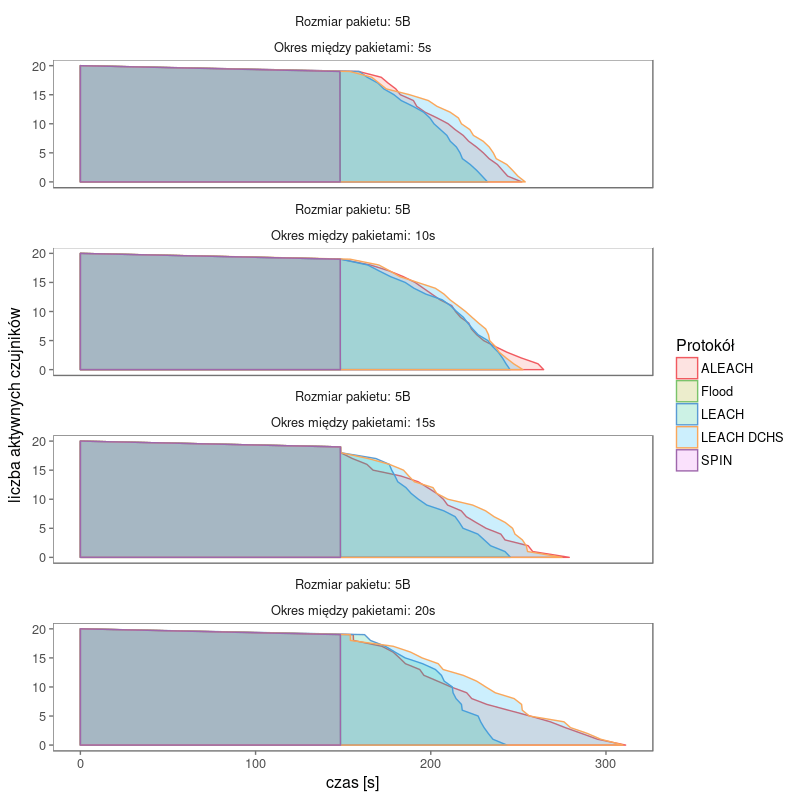
\includegraphics[scale=0.7]{\ImgPath/charts/alive_nodes_normal_20sensors_row1.png}
	\end{center}
	\caption{Aktywne węzły - 20 czujników, rozkład normalny, rozmiar pakietu: 5B}
\end{figure}

Przy rozmiarze pakietu 50B najlepszym protokołem z punktu widzenia całkowitej długości życia sieci okazał się ALEACH. W przypadku okresu między pakietami wynoszącym 20s zapewnił on około 50s dłuży czas działania sieci, jednakże protokoły LEACH oraz LEACH DCHS zapewniły dłuży okres jej stabilnego działania.

\begin{figure}[H]
	\begin{center}
		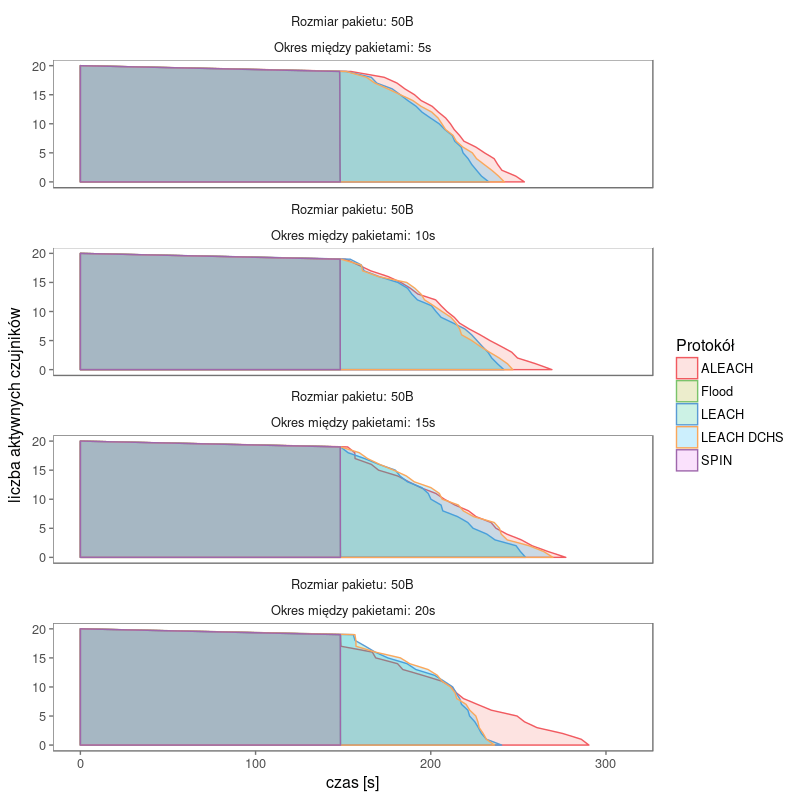
\includegraphics[scale=0.7]{\ImgPath/charts/alive_nodes_normal_20sensors_row2.png}
	\end{center}
	\caption{Aktywne węzły - 20 czujników, rozkład normalny, rozmiar pakietu: 50B}
\end{figure}

Przy rozmiarze pakietu 500B wśród protokołów umożliwiających najdłuższe działanie sieci znajduje się ALEACH. Przy okresie 10s LEACH działa lepiej od LEACH DCSH, a w przy okresie 5s i 20s LEACH DCSH działa dłużej niż LEACH.

\begin{figure}[H]
	\begin{center}
		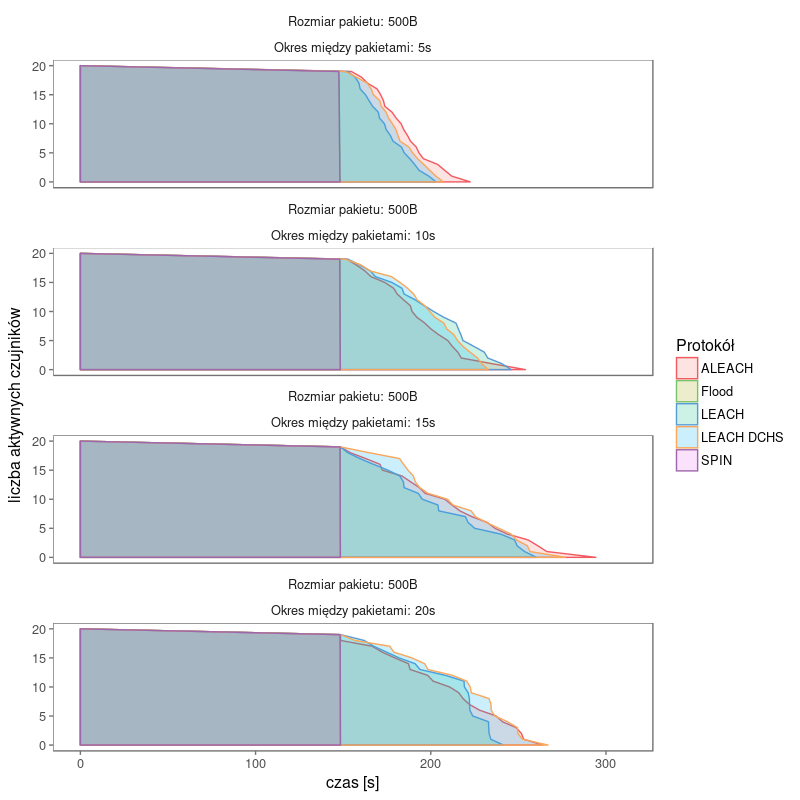
\includegraphics[scale=0.7]{\ImgPath/charts/alive_nodes_normal_20sensors_row3.png}
	\end{center}
	\caption{Aktywne węzły - 20 czujników, rozkład normalny, rozmiar pakietu: 500B}
\end{figure}

Przy rozmiarze pakietu 5000B jedynym przypadkiem w, którym ALEACH działa gorzej jest okres pomiędzy pakietami wynoszący 10s.

\begin{figure}[H]
	\begin{center}
		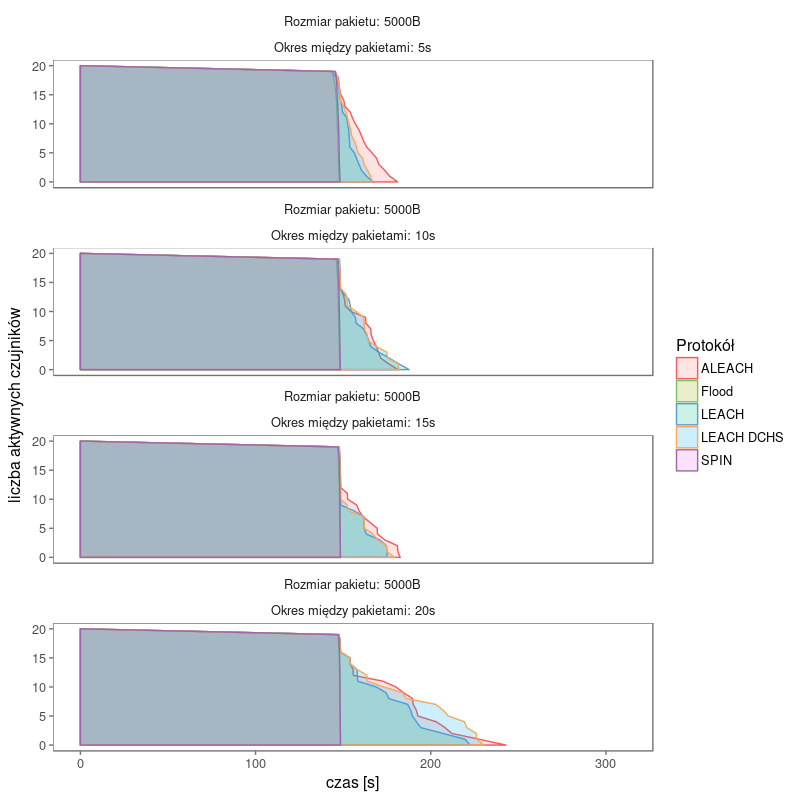
\includegraphics[scale=0.7]{\ImgPath/charts/alive_nodes_normal_20sensors_row4.png}
	\end{center}
	\caption{Aktywne węzły - 20 czujników, rozkład normalny, rozmiar pakietu: 5000B}
\end{figure}

\begin{figure}[H]
	\begin{center}
		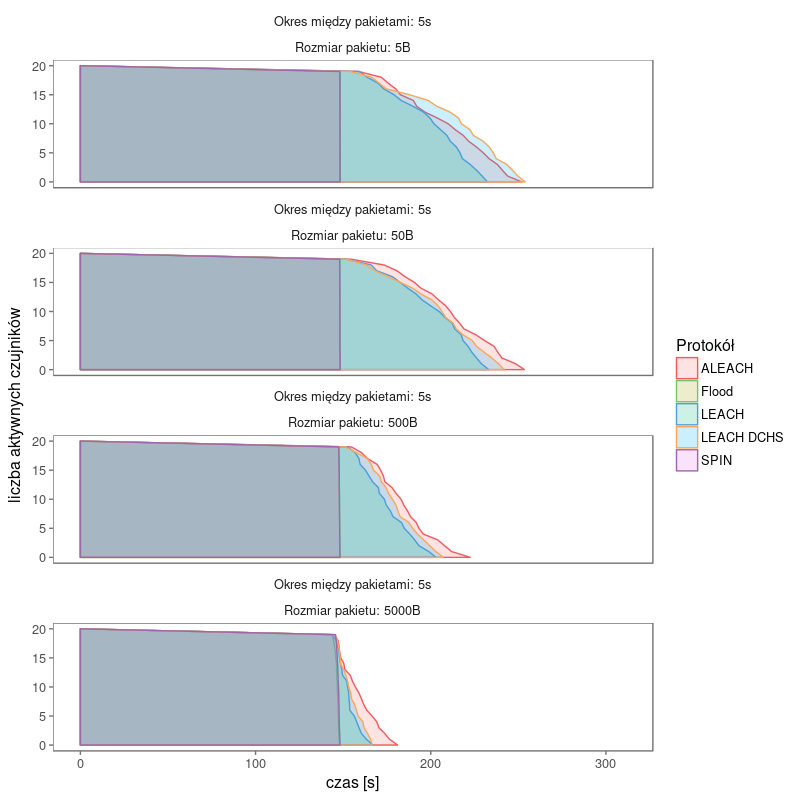
\includegraphics[scale=0.7]{\ImgPath/charts/alive_nodes_normal_20sensors_col1.png}
	\end{center}
	\caption{Aktywne węzły - 20 czujników, rozkład normalny, okres pomiędzy pakietami: 5s}
\end{figure}

\begin{figure}[H]
	\begin{center}
		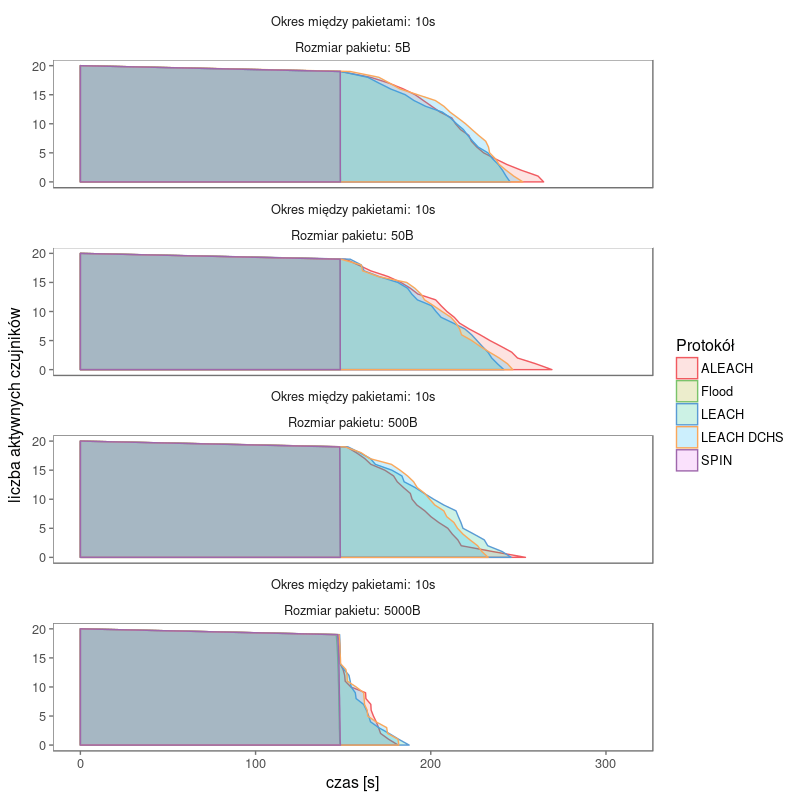
\includegraphics[scale=0.7]{\ImgPath/charts/alive_nodes_normal_20sensors_col2.png}
	\end{center}
	\caption{Aktywne węzły - 20 czujników, rozkład normalny, okres pomiędzy pakietami: 10s}
\end{figure}

\begin{figure}[H]
	\begin{center}
		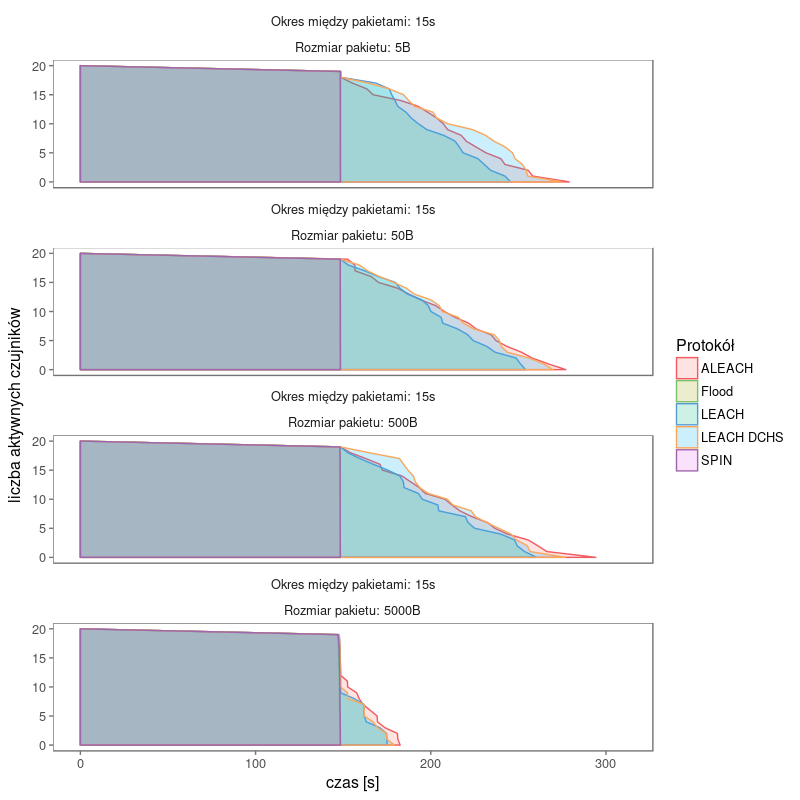
\includegraphics[scale=0.7]{\ImgPath/charts/alive_nodes_normal_20sensors_col3.png}
	\end{center}
	\caption{Aktywne węzły - 20 czujników, rozkład normalny, okres pomiędzy pakietami: 15s}
\end{figure}

\begin{figure}[H]
	\begin{center}
		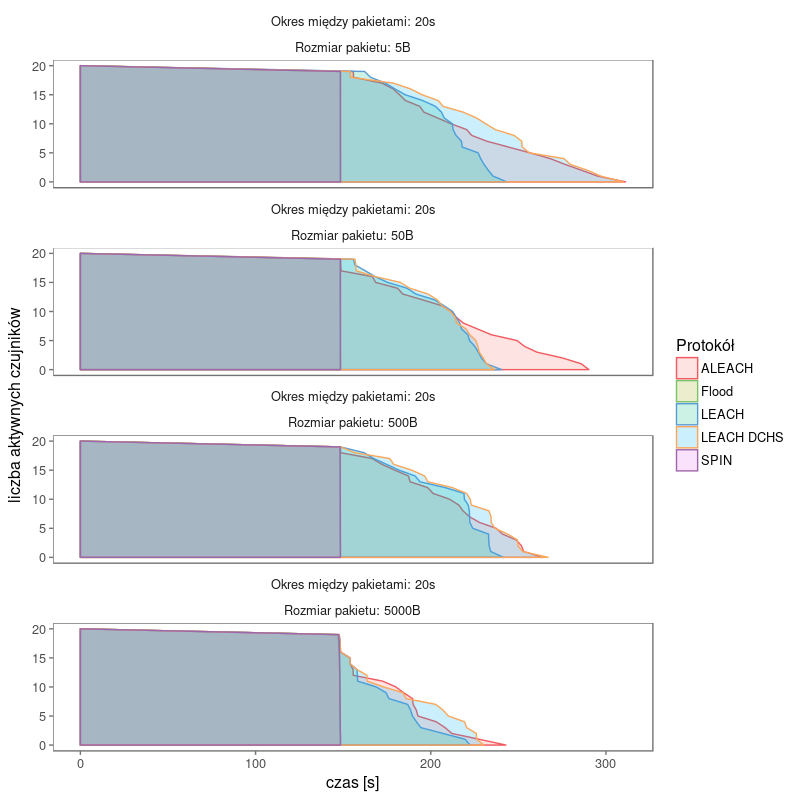
\includegraphics[scale=0.7]{\ImgPath/charts/alive_nodes_normal_20sensors_col4.png}
	\end{center}
	\caption{Aktywne węzły - 20 czujników, rozkład normalny, okres pomiędzy pakietami: 20s}
\end{figure}

\begin{figure}[H]
	\begin{center}
		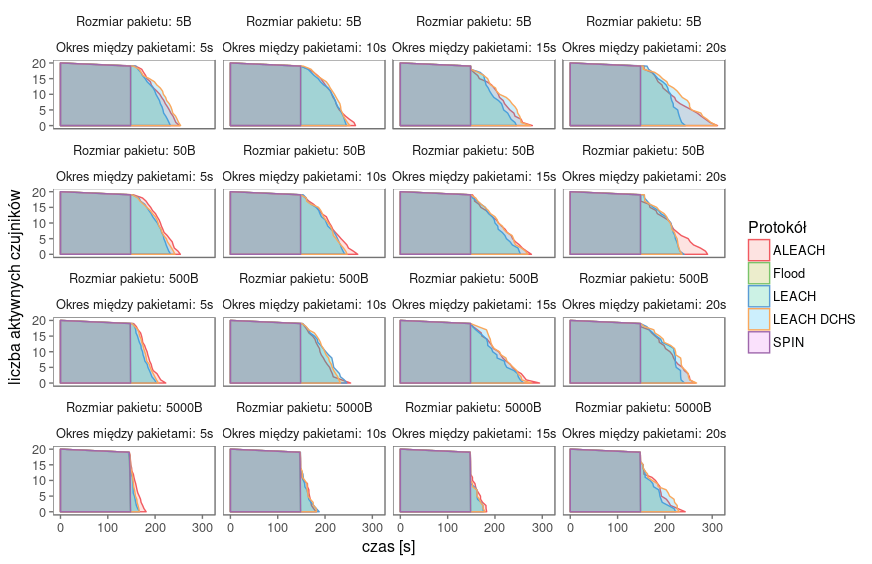
\includegraphics[scale=0.7]{\ImgPath/charts/alive_nodes_normal_20sensors.png}
	\end{center}
	\caption{Aktywne węzły - 20 czujników, rozkład normalny}
\end{figure}

Poniższe wykresy przedstawiają liczbę aktywnych węzłów sieci w czasie oraz w zależności od rozmiaru pakietu i odstępie czasu pomiędzy kolejnymi pakietami. Sieć składała się z dwustu węzłów, które rozmieszczone zostały zgodnie z rozkładem normalnym. Różnice pomiędzy wariantami protokołu LEACH są mniej wyraźne niż w przypadku sieci składającej się z dwudziestu węzłów. Najwrażliwszym na zmiany parametrów symulacji protokołem okazał się LEACH DCHS. Sieć go używająca działa wyraźnie krócej od pozostałych wariantów krótszych okresów pomiędzy pakietami oraz nieznacznie dłużej dla dłuższych okresów pomiędzy pakietami. Czas działania sieci dla protokołów Flood i SPIN podobnie jak w poprzednio pozostaje niezmienny, niezależnie od dobranych parametów wykresu.

\begin{figure}[!htbp]
	\begin{center}
		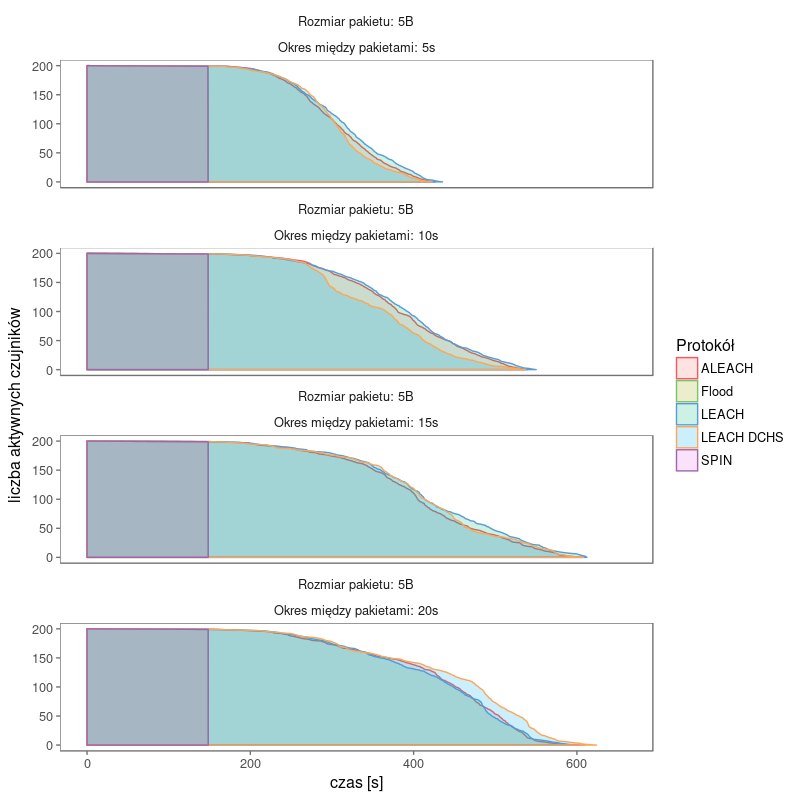
\includegraphics[scale=0.7]{\ImgPath/charts/alive_nodes_normal_200sensors_row1.png}
	\end{center}
	\caption{Aktywne węzły - 200 czujników, rozkład normalny, rozmiar pakietu: 5B}
\end{figure}

\begin{figure}[!htbp]
	\begin{center}
		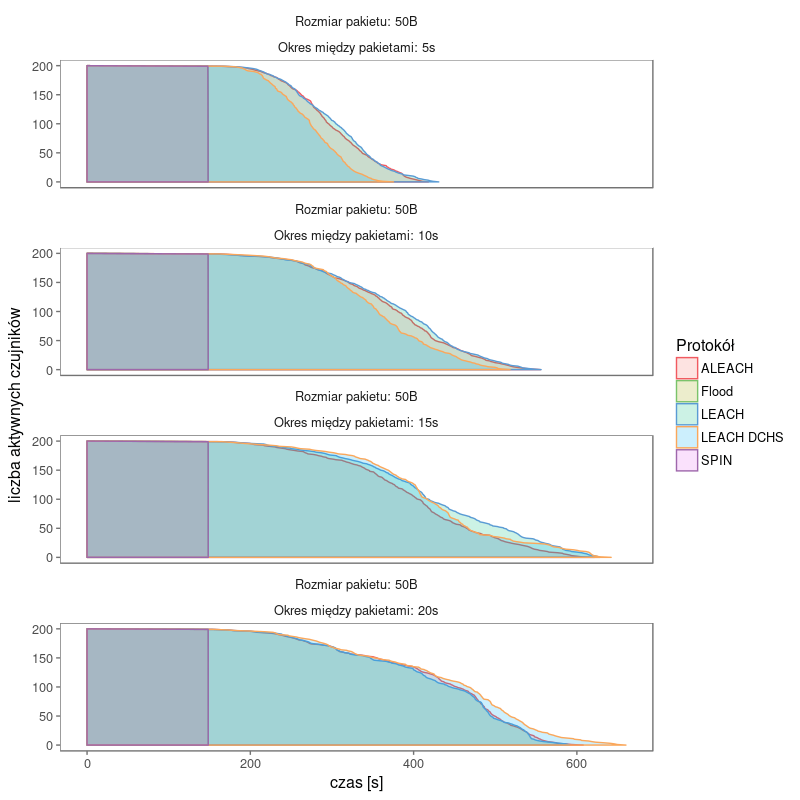
\includegraphics[scale=0.7]{\ImgPath/charts/alive_nodes_normal_200sensors_row2.png}
	\end{center}
	\caption{Aktywne węzły - 200 czujników, rozkład normalny, rozmiar pakietu: 50B}
\end{figure}

\begin{figure}[!htbp]
	\begin{center}
		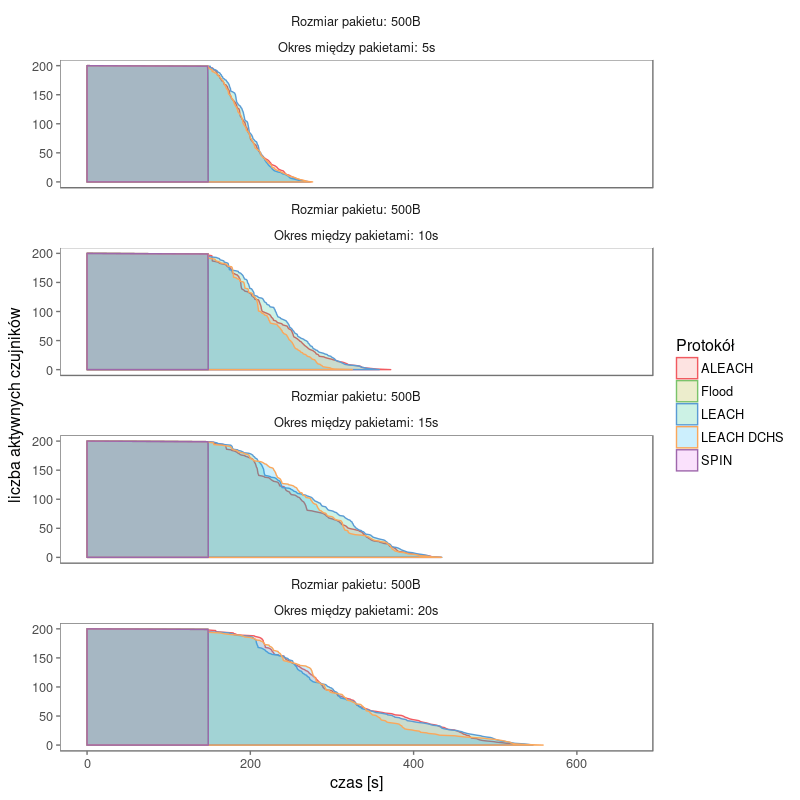
\includegraphics[scale=0.7]{\ImgPath/charts/alive_nodes_normal_200sensors_row3.png}
	\end{center}
	\caption{Aktywne węzły - 200 czujników, rozkład normalny, rozmiar pakietu: 500B}
\end{figure}

\begin{figure}[!htbp]
	\begin{center}
		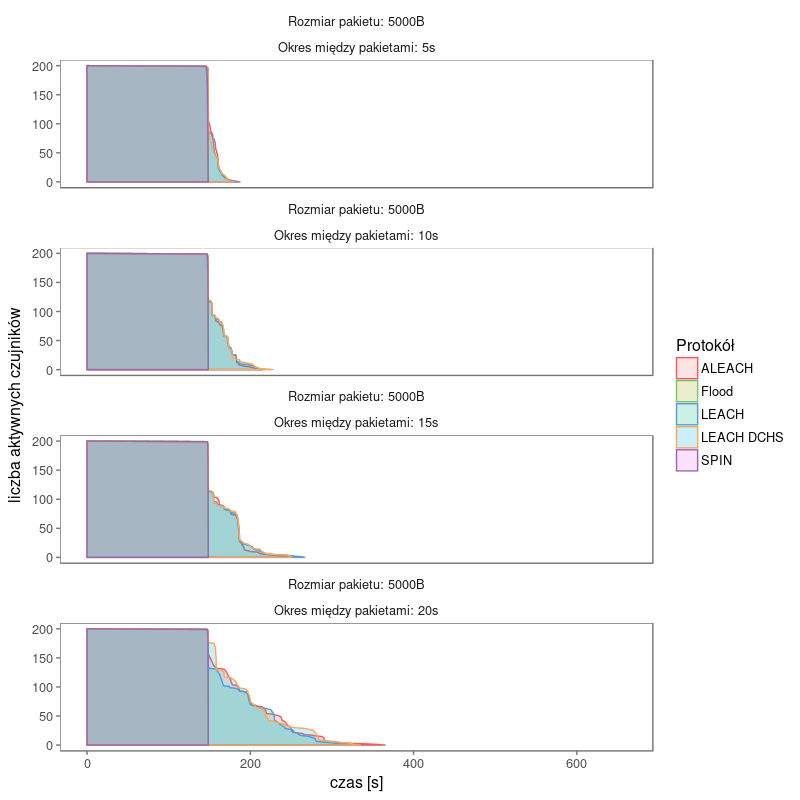
\includegraphics[scale=0.7]{\ImgPath/charts/alive_nodes_normal_200sensors_row4.png}
	\end{center}
	\caption{Aktywne węzły - 200 czujników, rozkład normalny, rozmiar pakietu: 5000B}
\end{figure}

\begin{figure}[!htbp]
	\begin{center}
		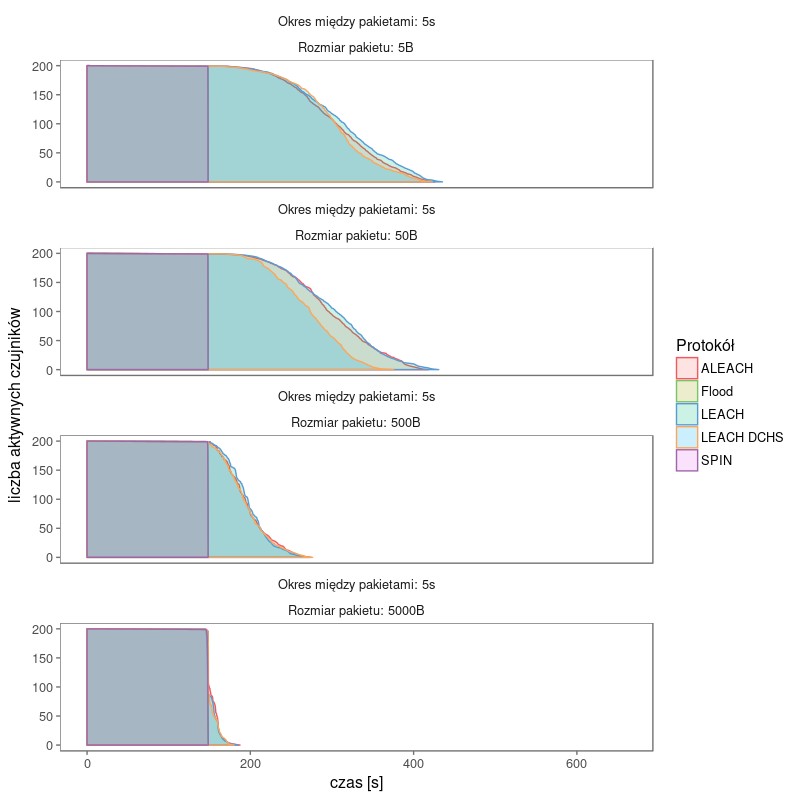
\includegraphics[scale=0.7]{\ImgPath/charts/alive_nodes_normal_200sensors_col1.png}
	\end{center}
	\caption{Aktywne węzły - 200 czujników, rozkład normalny, okres pomiędzy pakietami: 5s}
\end{figure}

\begin{figure}[!htbp]
	\begin{center}
		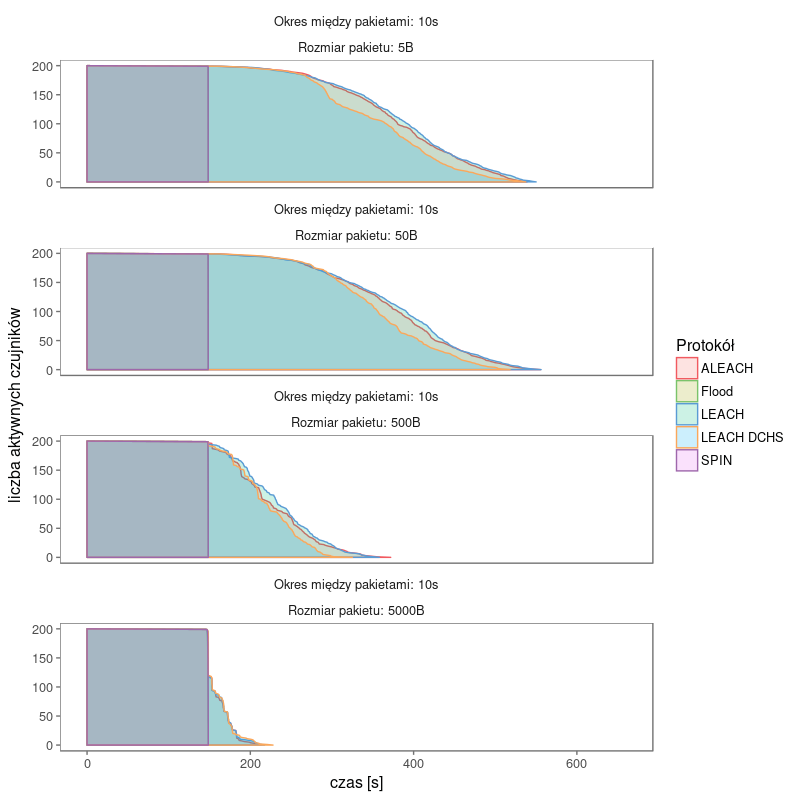
\includegraphics[scale=0.7]{\ImgPath/charts/alive_nodes_normal_200sensors_col2.png}
	\end{center}
	\caption{Aktywne węzły - 200 czujników, rozkład normalny, okres pomiędzy pakietami: 10s}
\end{figure}

\begin{figure}[!htbp]
	\begin{center}
		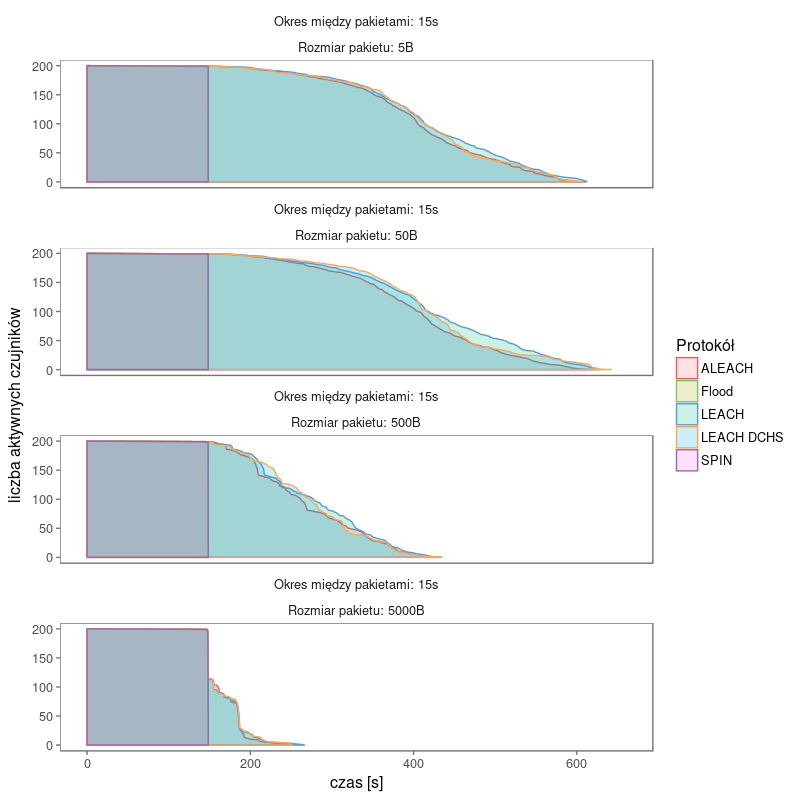
\includegraphics[scale=0.7]{\ImgPath/charts/alive_nodes_normal_200sensors_col3.png}
	\end{center}
	\caption{Aktywne węzły - 200 czujników, rozkład normalny, okres pomiędzy pakietami: 15s}
\end{figure}

\begin{figure}[!htbp]
	\begin{center}
		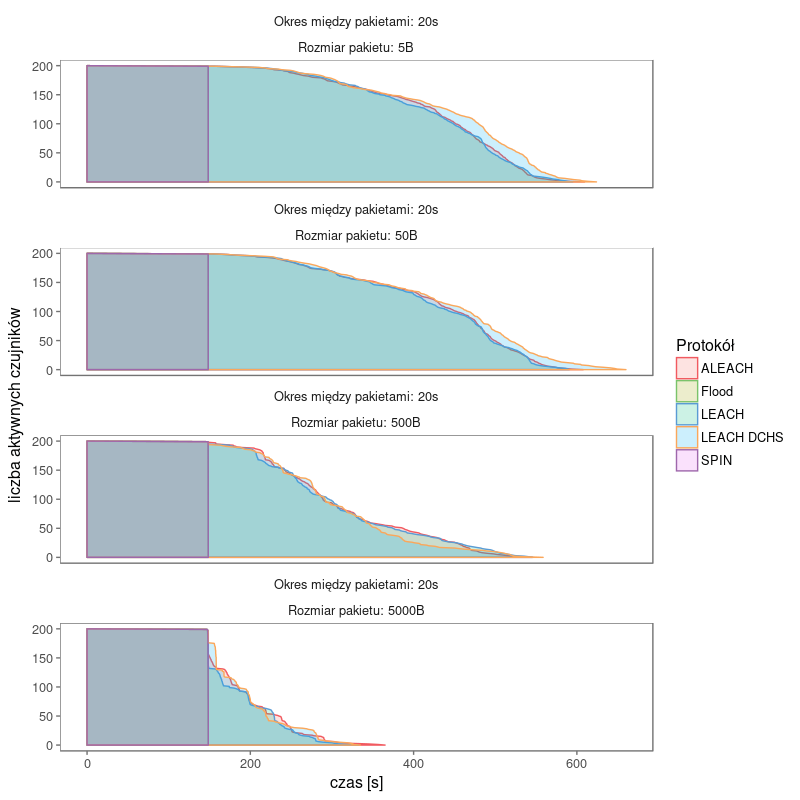
\includegraphics[scale=0.7]{\ImgPath/charts/alive_nodes_normal_200sensors_col4.png}
	\end{center}
	\caption{Aktywne węzły - 200 czujników, rozkład normalny, okres pomiędzy pakietami: 20s}
\end{figure}

\begin{figure}[!htbp]
	\begin{center}
		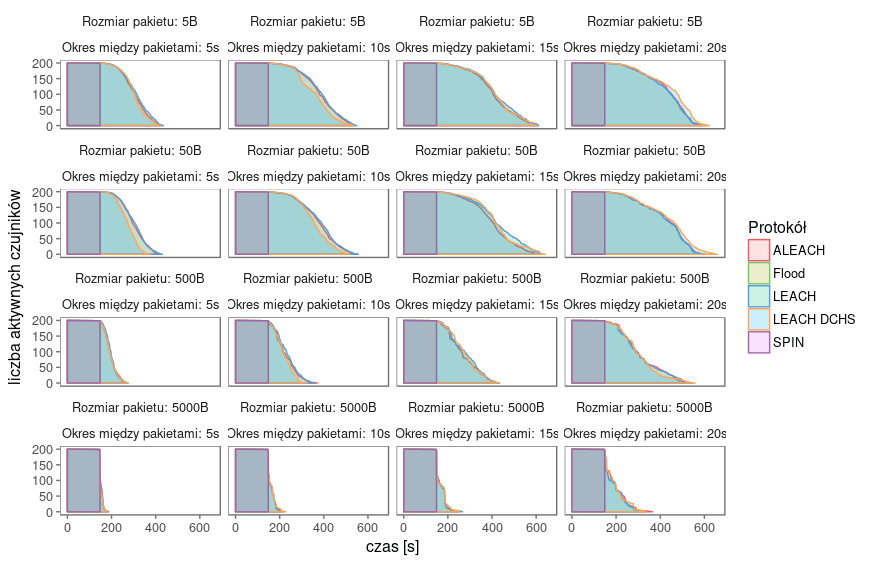
\includegraphics[scale=0.7]{\ImgPath/charts/alive_nodes_normal_200sensors.png}
	\end{center}
	\caption{Aktywne węzły - 200 czujników, rozkład normalny}
\end{figure}

\begin{figure}[!htbp]
	\begin{center}
		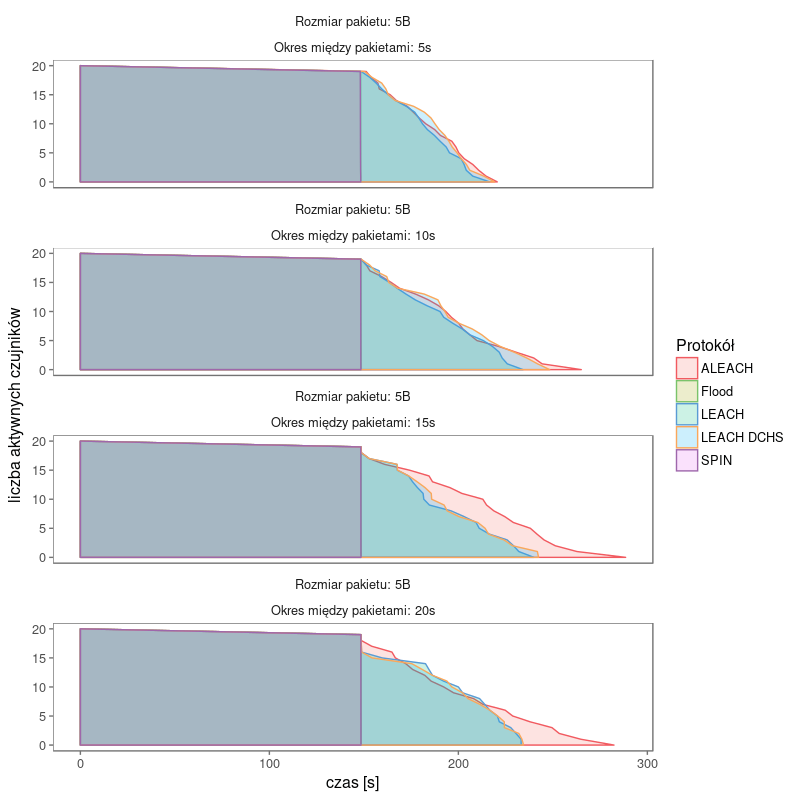
\includegraphics[scale=0.7]{\ImgPath/charts/alive_nodes_uniform_20sensors_row1.png}
	\end{center}
	\caption{Aktywne węzły - 20 czujników, rozkład jednorodny, rozmiar pakietu: 5B}
\end{figure}

\begin{figure}[!htbp]
	\begin{center}
		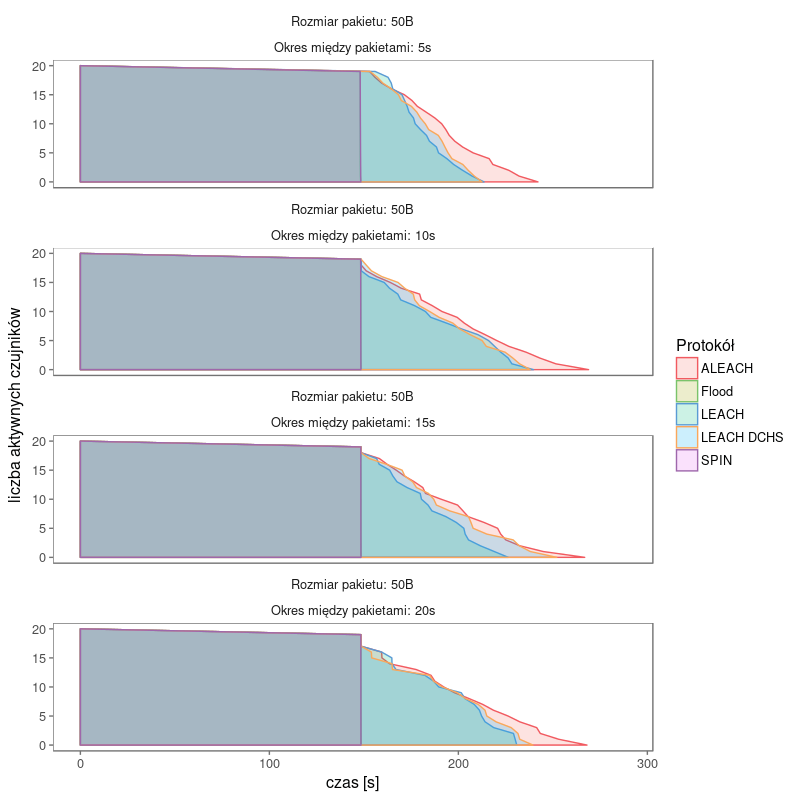
\includegraphics[scale=0.7]{\ImgPath/charts/alive_nodes_uniform_20sensors_row2.png}
	\end{center}
	\caption{Aktywne węzły - 20 czujników, rozkład jednorodny, rozmiar pakietu: 50B}
\end{figure}

\begin{figure}[!htbp]
	\begin{center}
		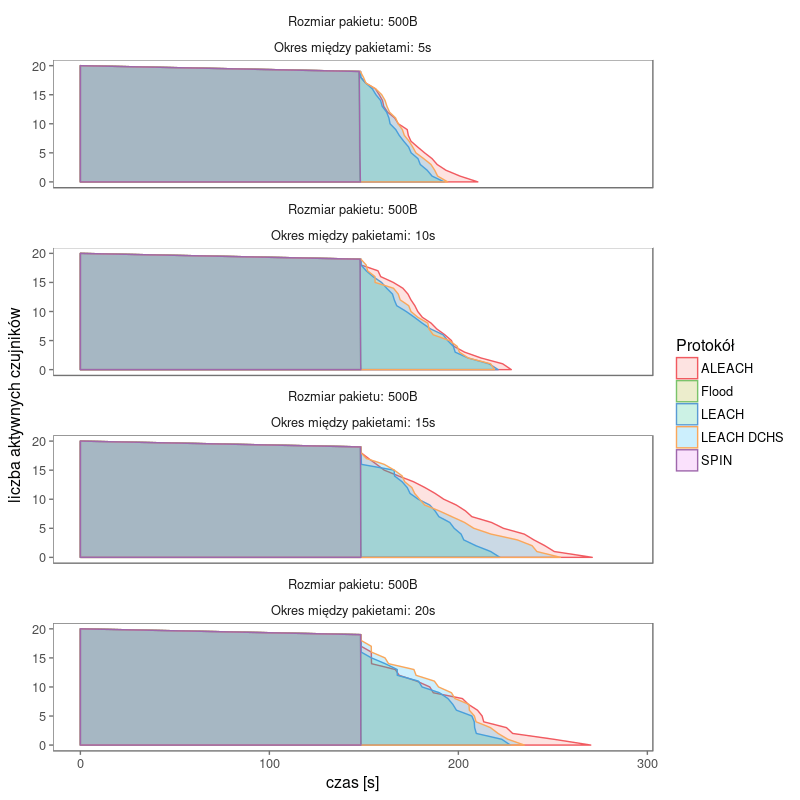
\includegraphics[scale=0.7]{\ImgPath/charts/alive_nodes_uniform_20sensors_row3.png}
	\end{center}
	\caption{Aktywne węzły - 20 czujników, rozkład jednorodny, rozmiar pakietu: 500B}
\end{figure}

\begin{figure}[!htbp]
	\begin{center}
		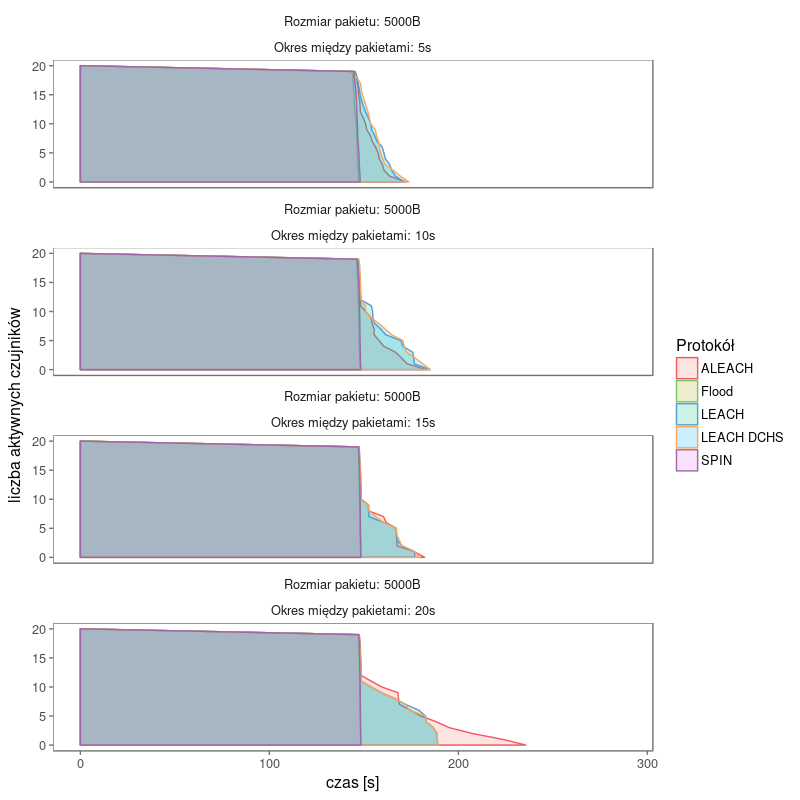
\includegraphics[scale=0.7]{\ImgPath/charts/alive_nodes_uniform_20sensors_row4.png}
	\end{center}
	\caption{Aktywne węzły - 20 czujników, rozkład jednorodny, rozmiar pakietu: 5000B}
\end{figure}

\begin{figure}[!htbp]
	\begin{center}
		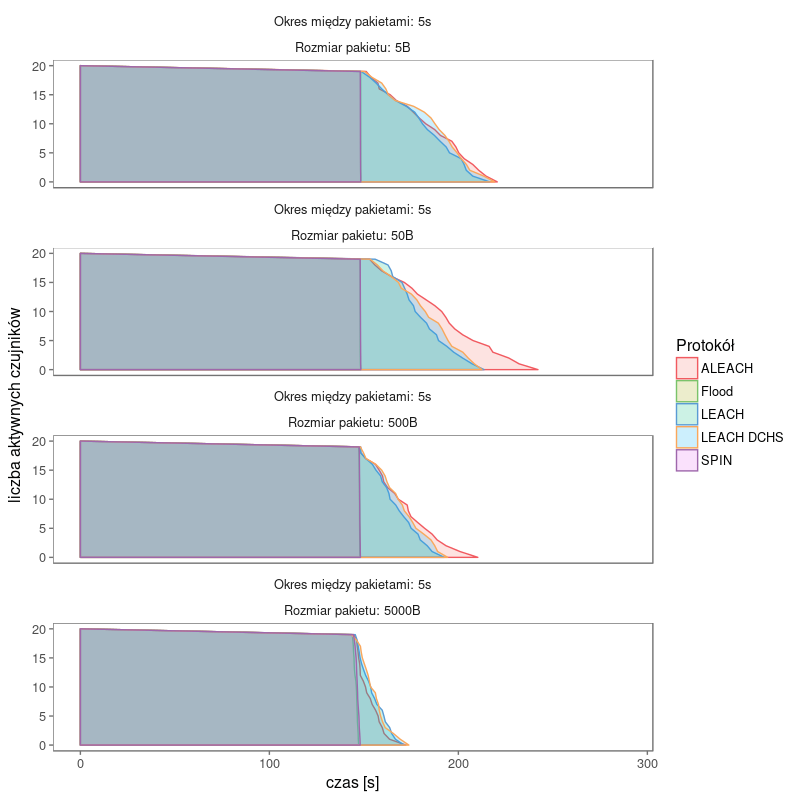
\includegraphics[scale=0.7]{\ImgPath/charts/alive_nodes_uniform_20sensors_col1.png}
	\end{center}
	\caption{Aktywne węzły - 20 czujników, rozkład jednorodny, okres pomiędzy pakietami: 5s}
\end{figure}

\begin{figure}[!htbp]
	\begin{center}
		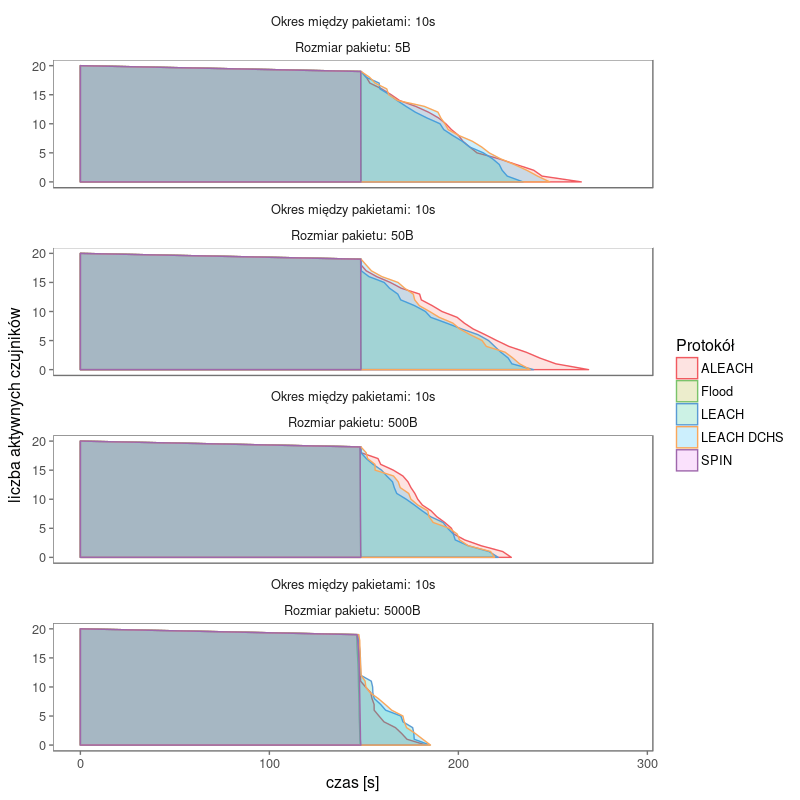
\includegraphics[scale=0.7]{\ImgPath/charts/alive_nodes_uniform_20sensors_col2.png}
	\end{center}
	\caption{Aktywne węzły - 20 czujników, rozkład jednorodny, okres pomiędzy pakietami: 10s}
\end{figure}

\begin{figure}[!htbp]
	\begin{center}
		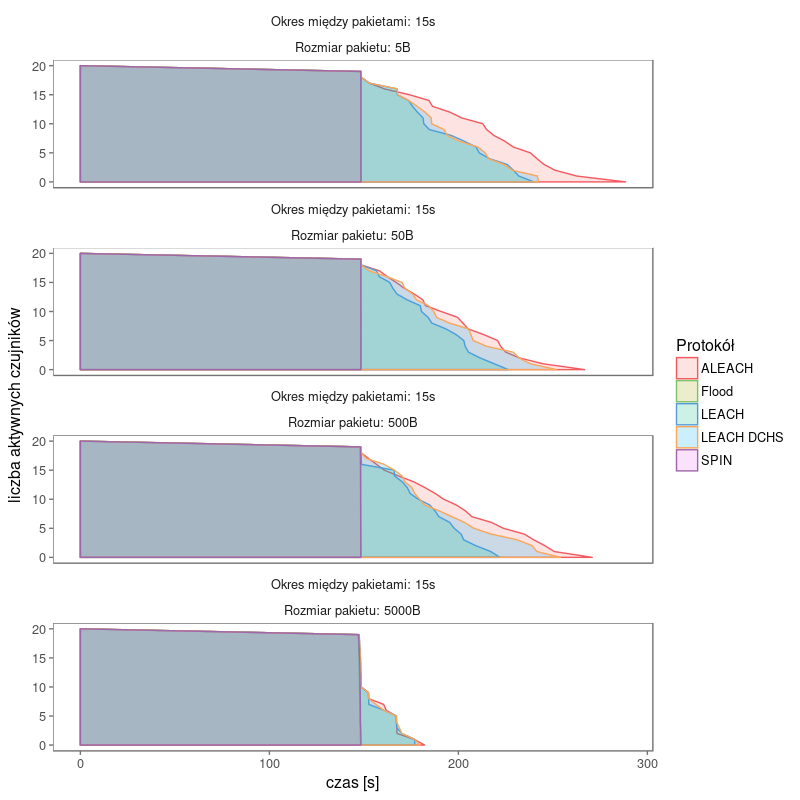
\includegraphics[scale=0.7]{\ImgPath/charts/alive_nodes_uniform_20sensors_col3.png}
	\end{center}
	\caption{Aktywne węzły - 20 czujników, rozkład jednorodny, okres pomiędzy pakietami: 15s}
\end{figure}

\begin{figure}[!htbp]
	\begin{center}
		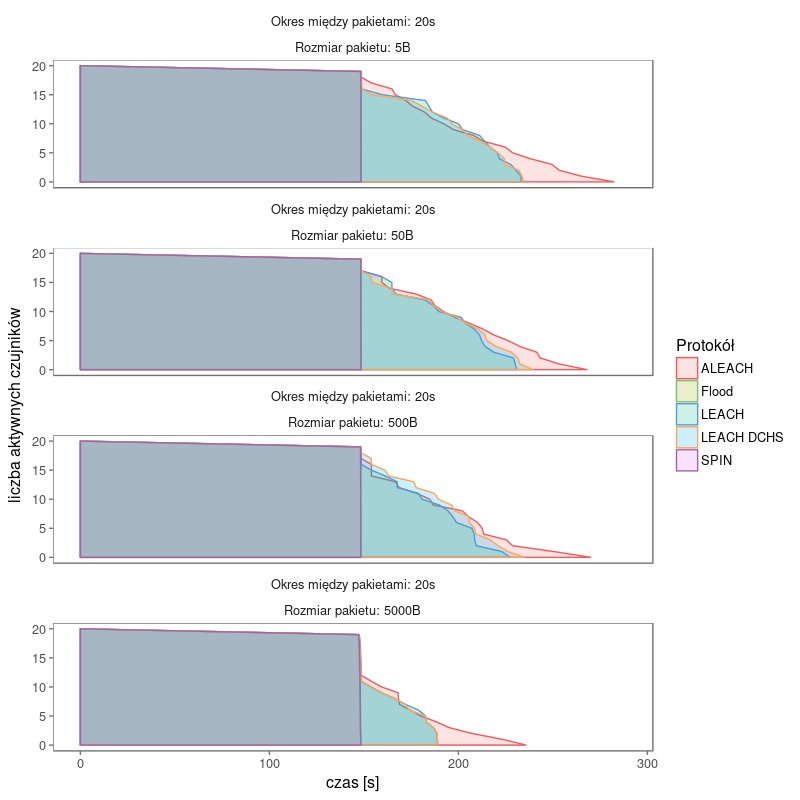
\includegraphics[scale=0.7]{\ImgPath/charts/alive_nodes_uniform_20sensors_col4.png}
	\end{center}
	\caption{Aktywne węzły - 20 czujników, rozkład jednorodny, okres pomiędzy pakietami: 20s}
\end{figure}

\begin{figure}[!htbp]
	\begin{center}
		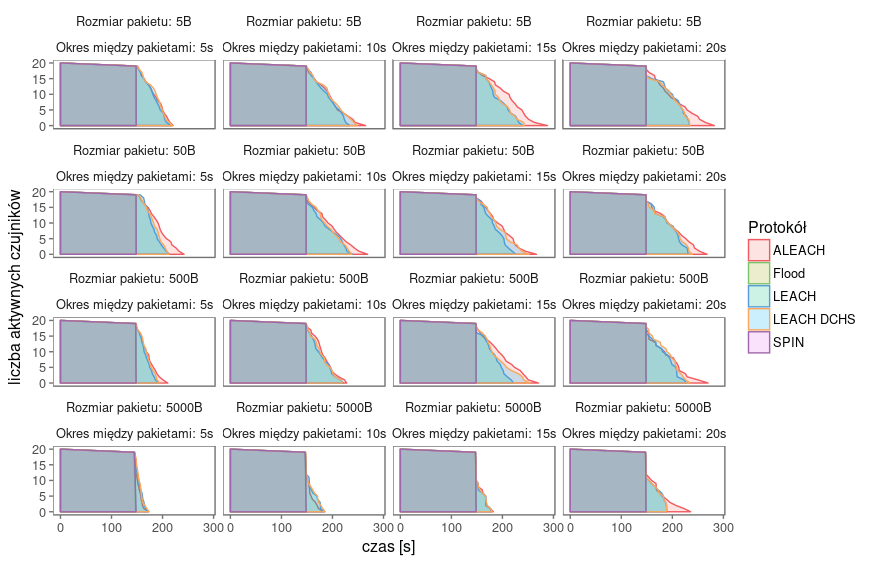
\includegraphics[scale=0.7]{\ImgPath/charts/alive_nodes_uniform_20sensors.png}
	\end{center}
	\caption{Aktywne węzły - 20 czujników, rozkład jednorodny}
\end{figure}

\begin{figure}[!htbp]
	\begin{center}
		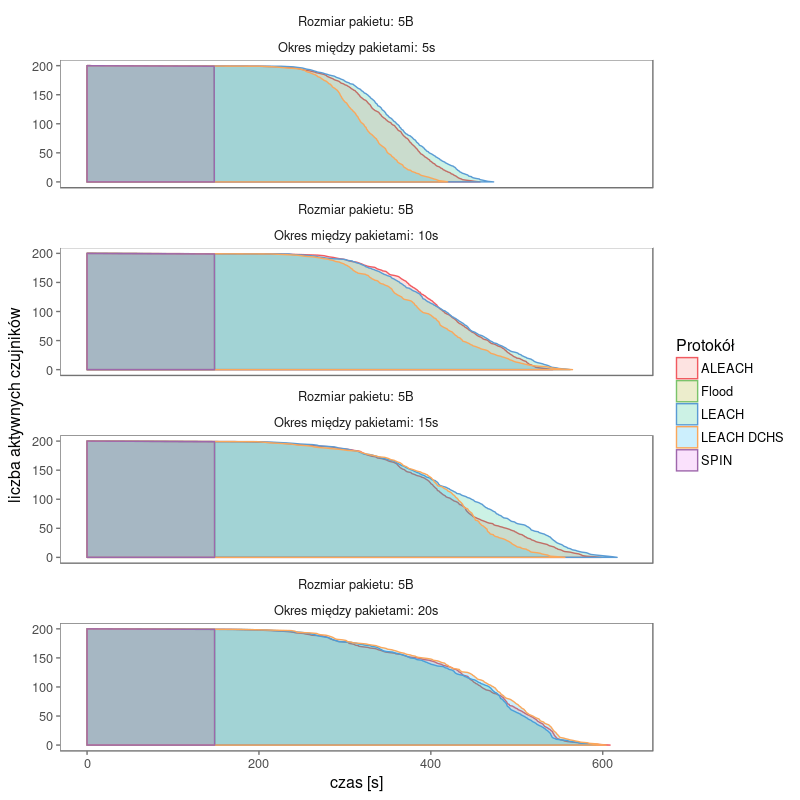
\includegraphics[scale=0.7]{\ImgPath/charts/alive_nodes_uniform_200sensors_row1.png}
	\end{center}
	\caption{Aktywne węzły - 200 czujników, rozkład jednorodny, rozmiar pakietu: 5B}
\end{figure}

\begin{figure}[!htbp]
	\begin{center}
		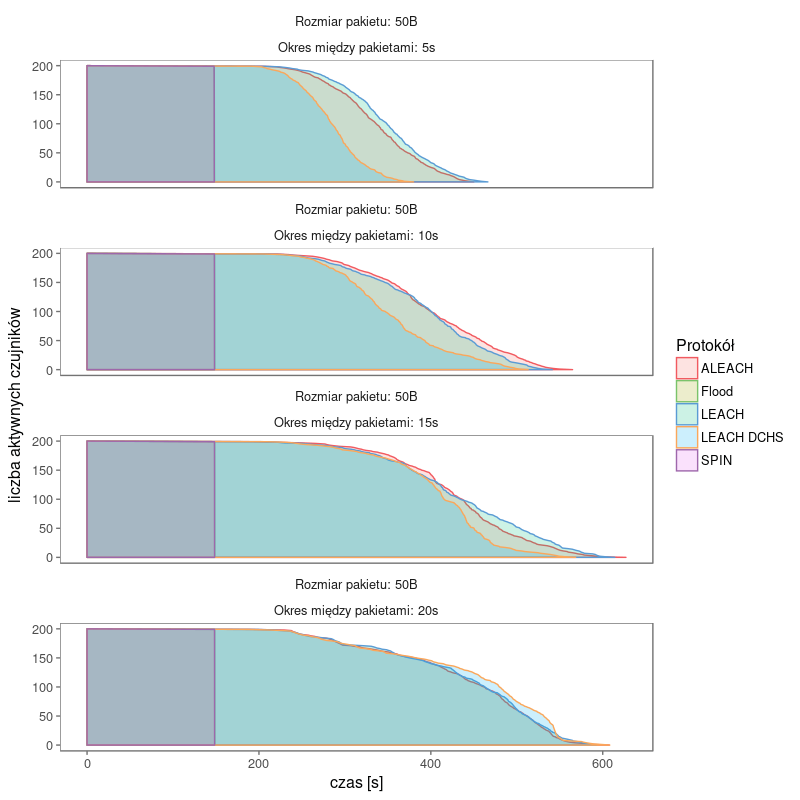
\includegraphics[scale=0.7]{\ImgPath/charts/alive_nodes_uniform_200sensors_row2.png}
	\end{center}
	\caption{Aktywne węzły - 200 czujników, rozkład jednorodny, rozmiar pakietu: 50B}
\end{figure}

\begin{figure}[!htbp]
	\begin{center}
		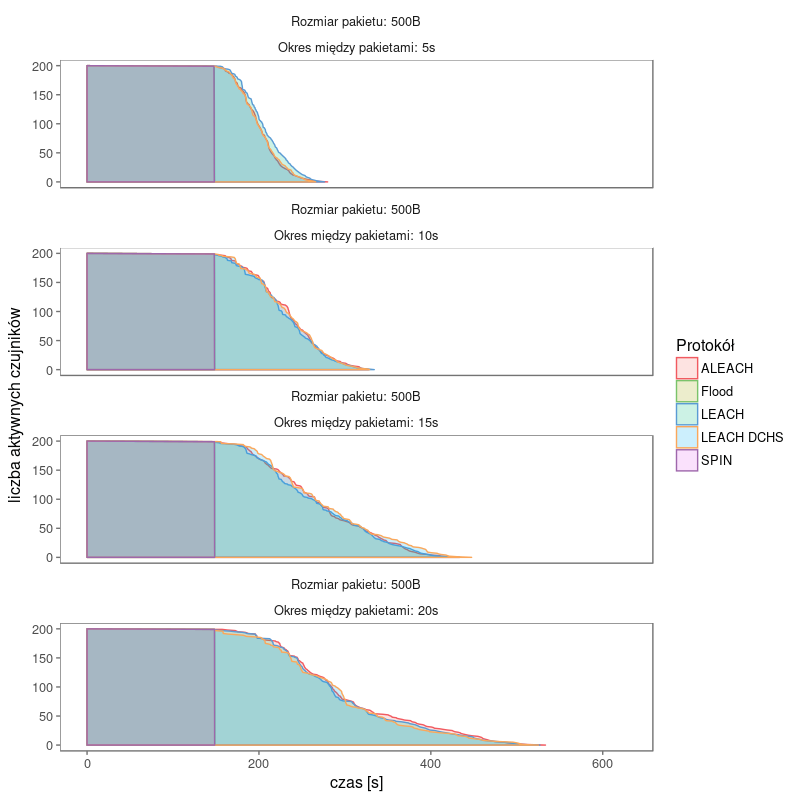
\includegraphics[scale=0.7]{\ImgPath/charts/alive_nodes_uniform_200sensors_row3.png}
	\end{center}
	\caption{Aktywne węzły - 200 czujników, rozkład jednorodny, rozmiar pakietu: 500B}
\end{figure}

\begin{figure}[!htbp]
	\begin{center}
		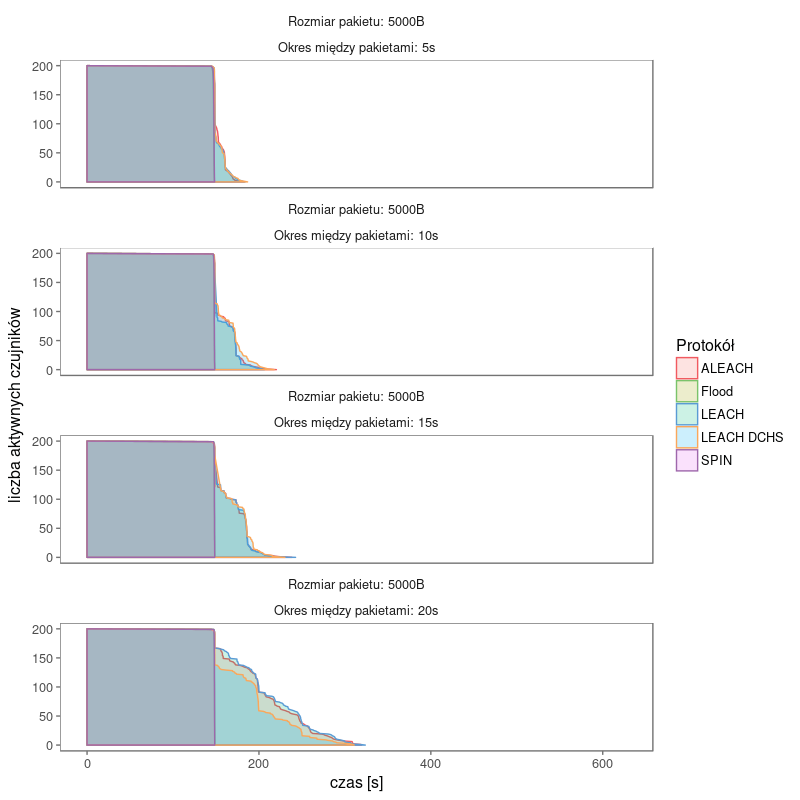
\includegraphics[scale=0.7]{\ImgPath/charts/alive_nodes_uniform_200sensors_row4.png}
	\end{center}
	\caption{Aktywne węzły - 200 czujników, rozkład jednorodny, rozmiar pakietu: 5000B}
\end{figure}

\begin{figure}[!htbp]
	\begin{center}
		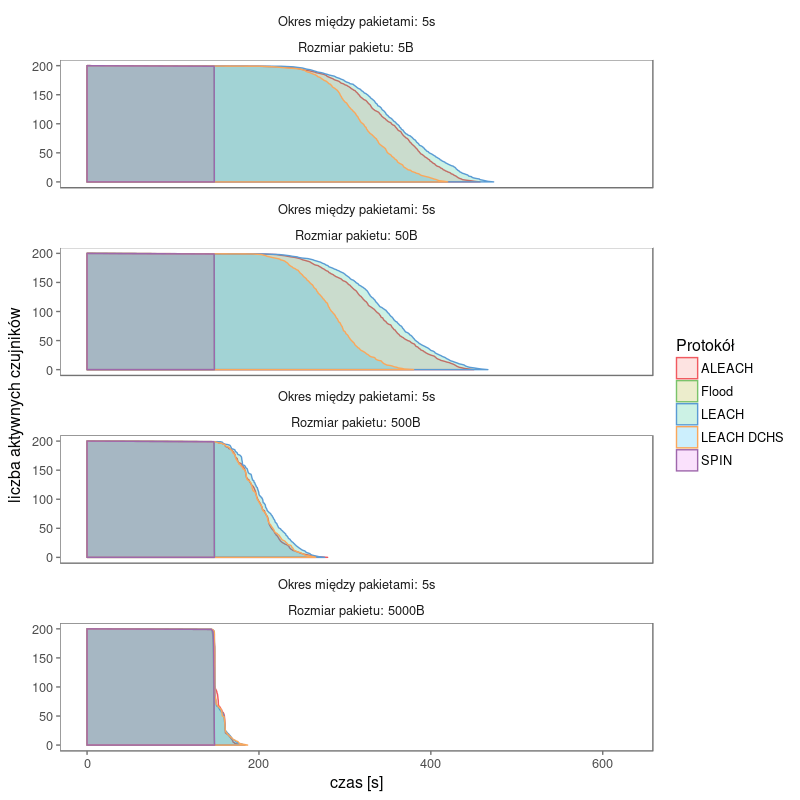
\includegraphics[scale=0.7]{\ImgPath/charts/alive_nodes_uniform_200sensors_col1.png}
	\end{center}
	\caption{Aktywne węzły - 200 czujników, rozkład jednorodny, okres pomiędzy pakietami: 5s}
\end{figure}

\begin{figure}[!htbp]
	\begin{center}
		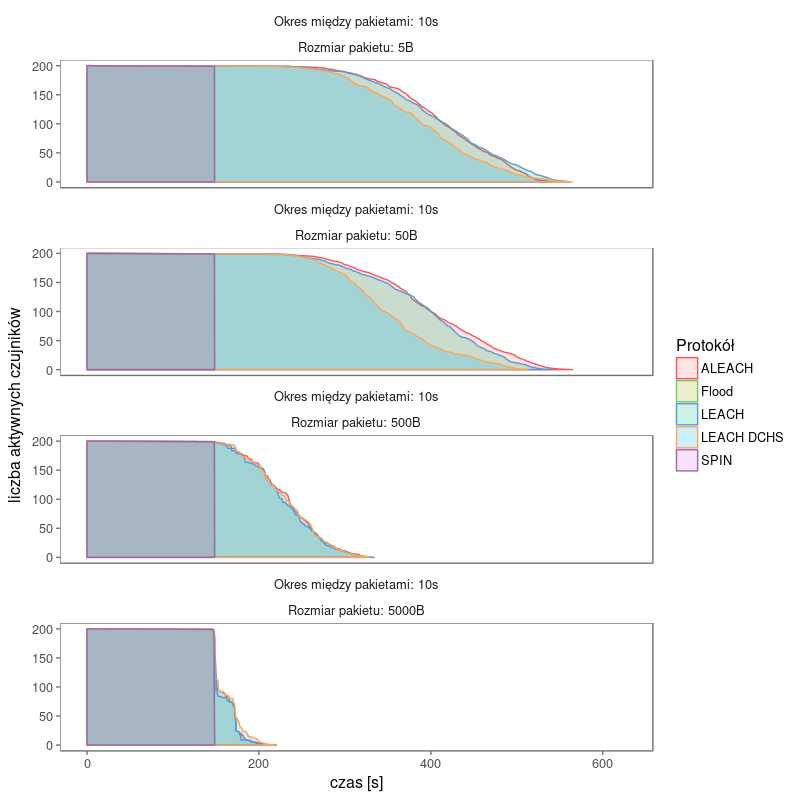
\includegraphics[scale=0.7]{\ImgPath/charts/alive_nodes_uniform_200sensors_col2.png}
	\end{center}
	\caption{Aktywne węzły - 200 czujników, rozkład jednorodny, okres pomiędzy pakietami: 10s}
\end{figure}

\begin{figure}[!htbp]
	\begin{center}
		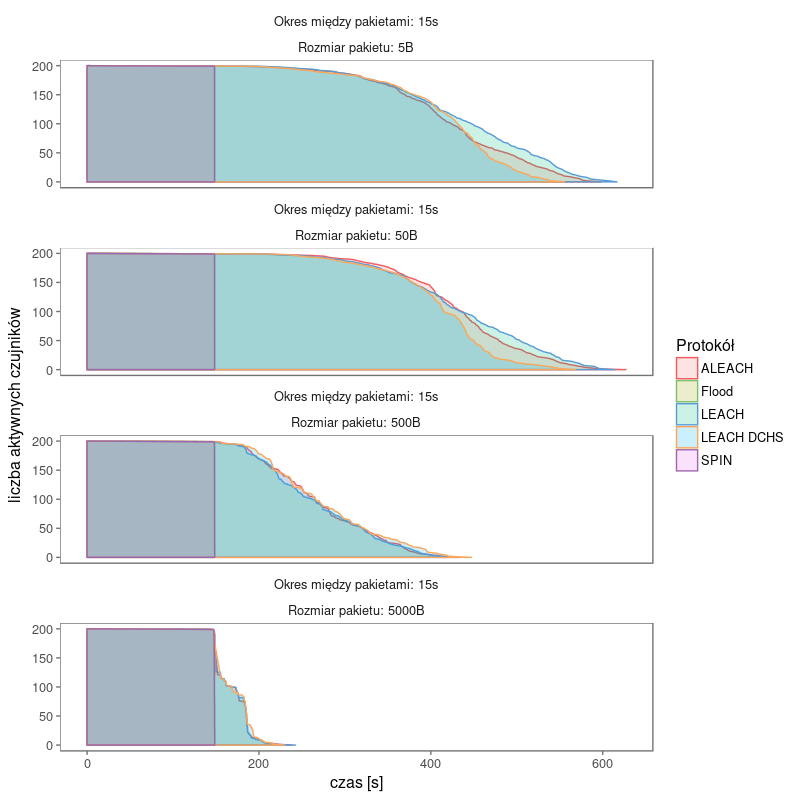
\includegraphics[scale=0.7]{\ImgPath/charts/alive_nodes_uniform_200sensors_col3.png}
	\end{center}
	\caption{Aktywne węzły - 200 czujników, rozkład jednorodny, okres pomiędzy pakietami: 15s}
\end{figure}

\begin{figure}[!htbp]
	\begin{center}
		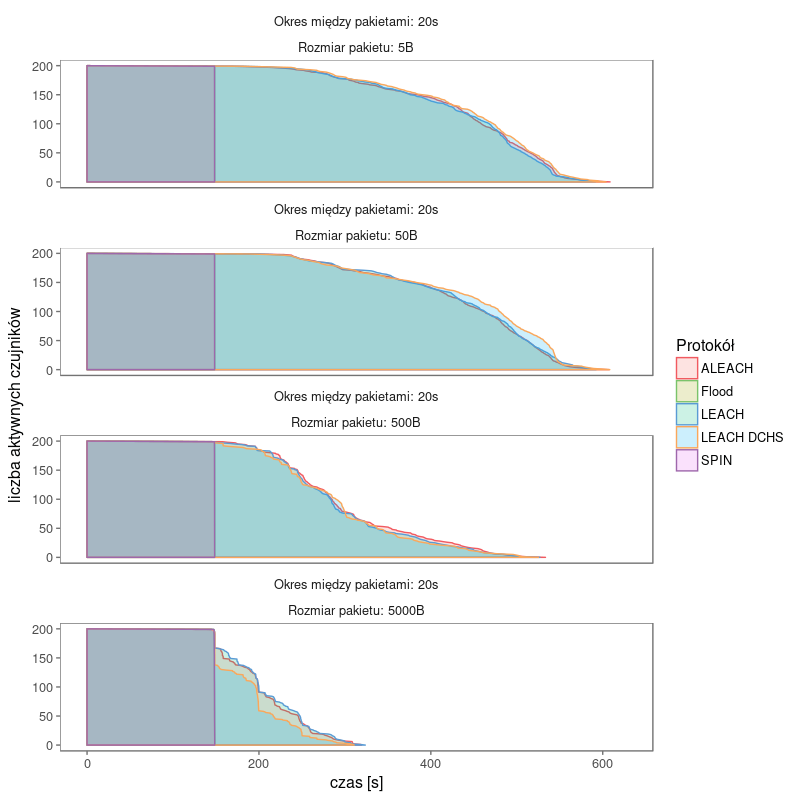
\includegraphics[scale=0.7]{\ImgPath/charts/alive_nodes_uniform_200sensors_col4.png}
	\end{center}
	\caption{Aktywne węzły - 200 czujników, rozkład jednorodny, okres pomiędzy pakietami: 20s}
\end{figure}

\begin{figure}[!htbp]
	\begin{center}
		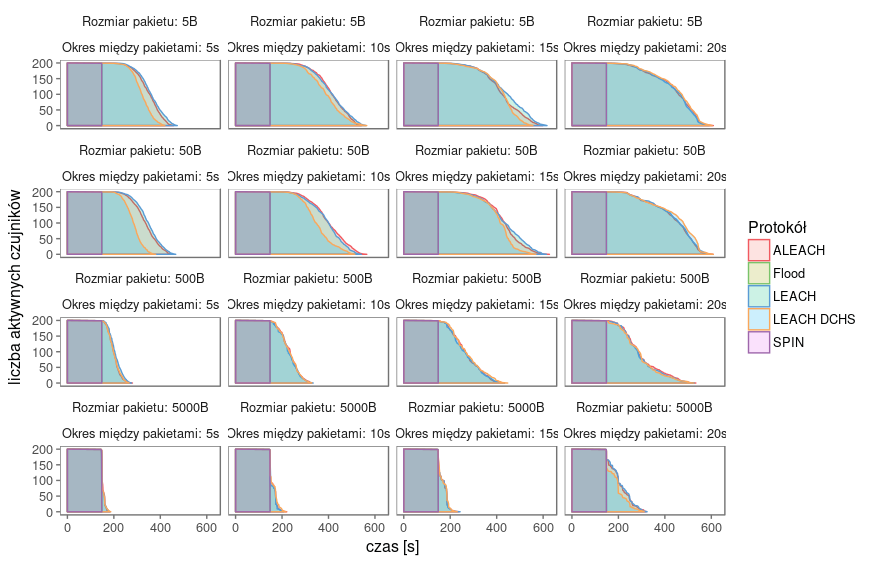
\includegraphics[scale=0.7]{\ImgPath/charts/alive_nodes_uniform_200sensors.png}
	\end{center}
	\caption{Aktywne węzły - 200 czujników, rozkład jednorodny}
\end{figure}


\subsection{Energia}

\begin{figure}[!htbp]
	\begin{center}
		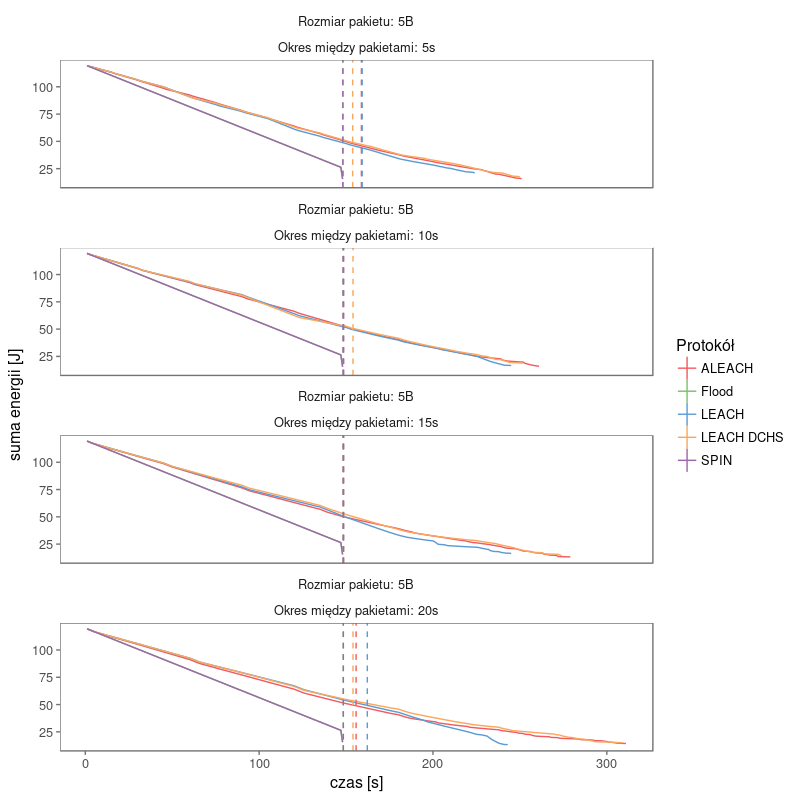
\includegraphics[scale=0.7]{\ImgPath/charts/stored_energy_normal_20sensors_row1.png}
	\end{center}
	\caption{Energia sieci - 20 czujników, rozkład normalny, rozmiar pakietu: 5B}
\end{figure}

\begin{figure}[!htbp]
	\begin{center}
		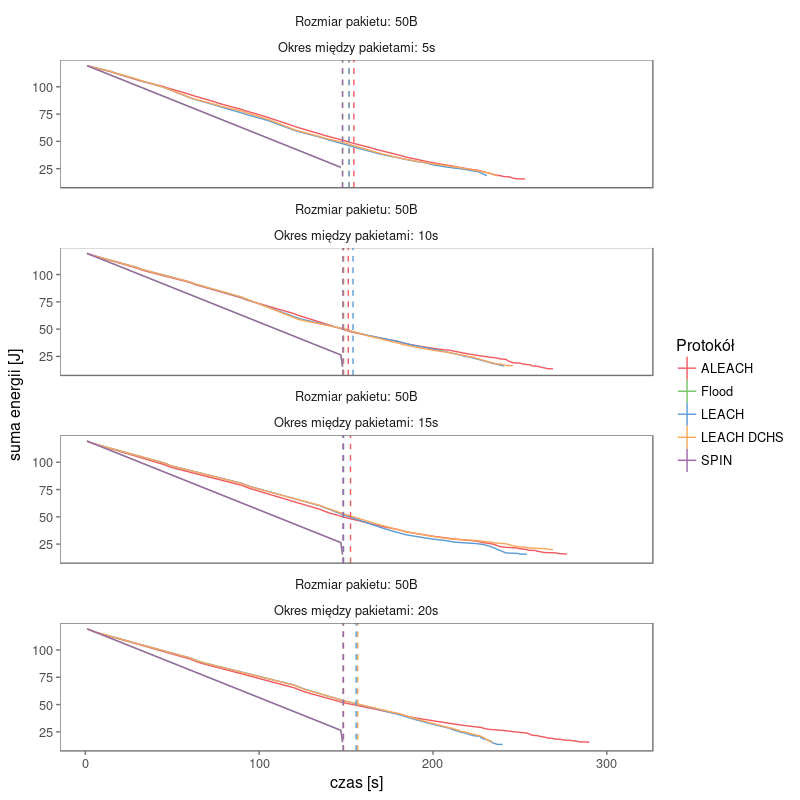
\includegraphics[scale=0.7]{\ImgPath/charts/stored_energy_normal_20sensors_row2.png}
	\end{center}
	\caption{Energia sieci - 20 czujników, rozkład normalny, rozmiar pakietu: 50B}
\end{figure}

\begin{figure}[!htbp]
	\begin{center}
		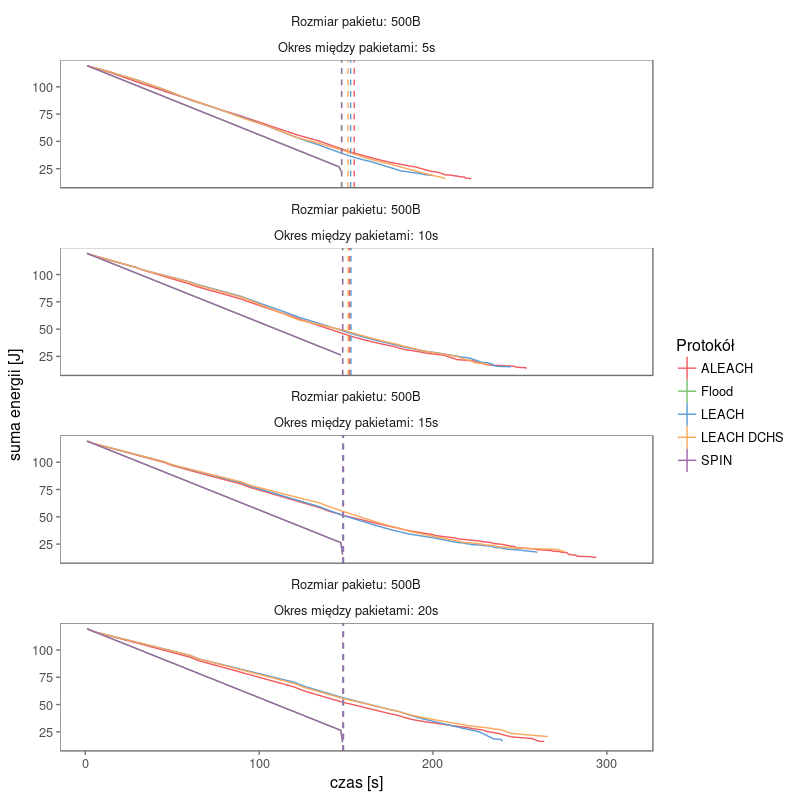
\includegraphics[scale=0.7]{\ImgPath/charts/stored_energy_normal_20sensors_row3.png}
	\end{center}
	\caption{Energia sieci - 20 czujników, rozkład normalny, rozmiar pakietu: 500B}
\end{figure}

\begin{figure}[!htbp]
	\begin{center}
		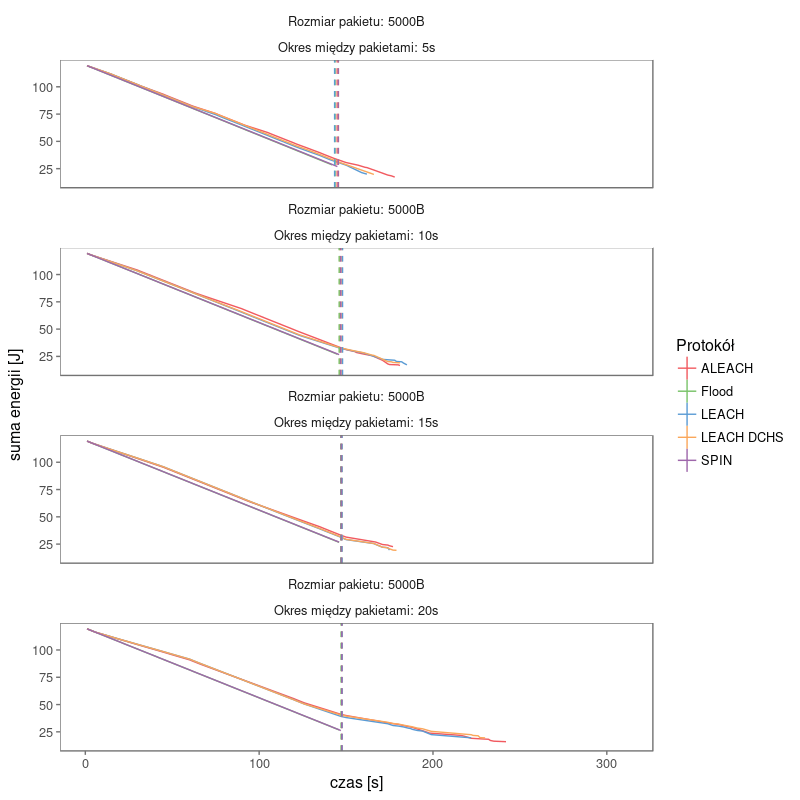
\includegraphics[scale=0.7]{\ImgPath/charts/stored_energy_normal_20sensors_row4.png}
	\end{center}
	\caption{Energia sieci - 20 czujników, rozkład normalny, rozmiar pakietu: 5000B}
\end{figure}

\begin{figure}[!htbp]
	\begin{center}
		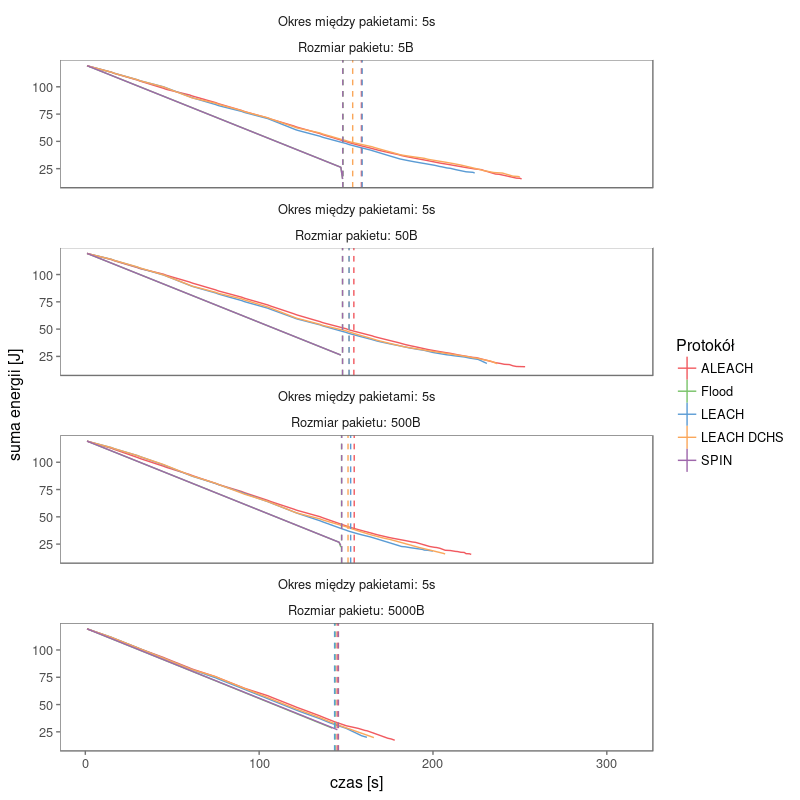
\includegraphics[scale=0.7]{\ImgPath/charts/stored_energy_normal_20sensors_col1.png}
	\end{center}
	\caption{Energia sieci - 20 czujników, rozkład normalny, okres pomiędzy pakietami: 5s}
\end{figure}

\begin{figure}[!htbp]
	\begin{center}
		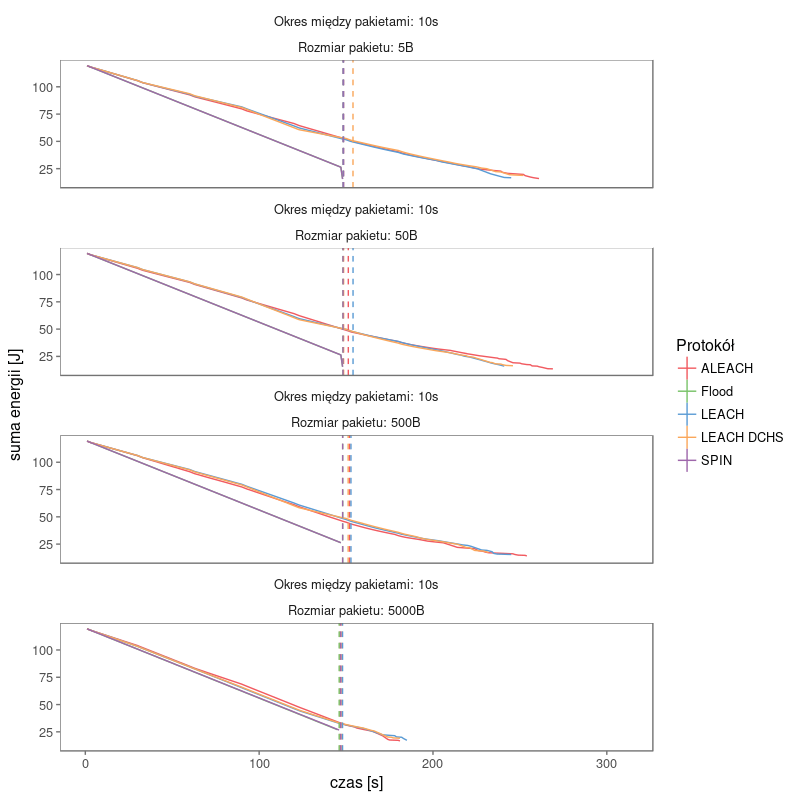
\includegraphics[scale=0.7]{\ImgPath/charts/stored_energy_normal_20sensors_col2.png}
	\end{center}
	\caption{Energia sieci - 20 czujników, rozkład normalny, okres pomiędzy pakietami: 10s}
\end{figure}

\begin{figure}[!htbp]
	\begin{center}
		\includegraphics[scale=0.7]{\ImgPath/charts/stored_energy_normal_20sensors_col3.png}
	\end{center}
	\caption{Energia sieci - 20 czujników, rozkład normalny, okres pomiędzy pakietami: 15s}
\end{figure}

\begin{figure}[!htbp]
	\begin{center}
		\includegraphics[scale=0.7]{\ImgPath/charts/stored_energy_normal_20sensors_col4.png}
	\end{center}
	\caption{Energia sieci - 20 czujników, rozkład normalny, okres pomiędzy pakietami: 20s}
\end{figure}

\begin{figure}[!htbp]
	\begin{center}
		\includegraphics[scale=0.7]{\ImgPath/charts/stored_energy_normal_20sensors.png}
	\end{center}
	\caption{Energia sieci - 20 czujników, rozkład normalny}
\end{figure}

\begin{figure}[H]
	\begin{center}
		\includegraphics[scale=0.7]{\ImgPath/charts/stored_energy_normal_200sensors_row1.png}
	\end{center}
	\caption{Energia sieci - 200 czujników, rozkład normalny, rozmiar pakietu: 5B}
\end{figure}

\begin{figure}[H]
	\begin{center}
		\includegraphics[scale=0.7]{\ImgPath/charts/stored_energy_normal_200sensors_row2.png}
	\end{center}
	\caption{Energia sieci - 200 czujników, rozkład normalny, rozmiar pakietu: 50B}
\end{figure}

\begin{figure}[H]
	\begin{center}
		\includegraphics[scale=0.7]{\ImgPath/charts/stored_energy_normal_200sensors_row3.png}
	\end{center}
	\caption{Energia sieci - 200 czujników, rozkład normalny, rozmiar pakietu: 500B}
\end{figure}

\begin{figure}[H]
	\begin{center}
		\includegraphics[scale=0.7]{\ImgPath/charts/stored_energy_normal_200sensors_row4.png}
	\end{center}
	\caption{Energia sieci - 200 czujników, rozkład normalny, rozmiar pakietu: 5000B}
\end{figure}

\begin{figure}[H]
	\begin{center}
		\includegraphics[scale=0.7]{\ImgPath/charts/stored_energy_normal_200sensors_col1.png}
	\end{center}
	\caption{Energia sieci - 200 czujników, rozkład normalny, okres pomiędzy pakietami: 5s}
\end{figure}

\begin{figure}[H]
	\begin{center}
		\includegraphics[scale=0.7]{\ImgPath/charts/stored_energy_normal_200sensors_col2.png}
	\end{center}
	\caption{Energia sieci - 200 czujników, rozkład normalny, okres pomiędzy pakietami: 10s}
\end{figure}

\begin{figure}[H]
	\begin{center}
		\includegraphics[scale=0.7]{\ImgPath/charts/stored_energy_normal_200sensors_col3.png}
	\end{center}
	\caption{Energia sieci - 200 czujników, rozkład normalny, okres pomiędzy pakietami: 15s}
\end{figure}

\begin{figure}[H]
	\begin{center}
		\includegraphics[scale=0.7]{\ImgPath/charts/stored_energy_normal_200sensors_col4.png}
	\end{center}
	\caption{Energia sieci - 200 czujników, rozkład normalny, okres pomiędzy pakietami: 20s}
\end{figure}

\begin{figure}[H]
	\begin{center}
		\includegraphics[scale=0.7]{\ImgPath/charts/stored_energy_normal_200sensors.png}
	\end{center}
	\caption{Energia sieci - 200 czujników, rozkład normalny}
\end{figure}

\begin{figure}[H]
	\begin{center}
		\includegraphics[scale=0.7]{\ImgPath/charts/stored_energy_uniform_20sensors_row1.png}
	\end{center}
	\caption{Energia sieci - 20 czujników, rozkład jednorodny, rozmiar pakietu: 5B}
\end{figure}

\begin{figure}[H]
	\begin{center}
		\includegraphics[scale=0.7]{\ImgPath/charts/stored_energy_uniform_20sensors_row2.png}
	\end{center}
	\caption{Energia sieci - 20 czujników, rozkład jednorodny, rozmiar pakietu: 50B}
\end{figure}

\begin{figure}[H]
	\begin{center}
		\includegraphics[scale=0.7]{\ImgPath/charts/stored_energy_uniform_20sensors_row3.png}
	\end{center}
	\caption{Energia sieci - 20 czujników, rozkład jednorodny, rozmiar pakietu: 500B}
\end{figure}

\begin{figure}[H]
	\begin{center}
		\includegraphics[scale=0.7]{\ImgPath/charts/stored_energy_uniform_20sensors_row4.png}
	\end{center}
	\caption{Energia sieci - 20 czujników, rozkład jednorodny, rozmiar pakietu: 5000B}
\end{figure}

\begin{figure}[H]
	\begin{center}
		\includegraphics[scale=0.7]{\ImgPath/charts/stored_energy_uniform_20sensors_col1.png}
	\end{center}
	\caption{Energia sieci - 20 czujników, rozkład jednorodny, okres pomiędzy pakietami: 5s}
\end{figure}

\begin{figure}[H]
	\begin{center}
		\includegraphics[scale=0.7]{\ImgPath/charts/stored_energy_uniform_20sensors_col2.png}
	\end{center}
	\caption{Energia sieci - 20 czujników, rozkład jednorodny, okres pomiędzy pakietami: 10s}
\end{figure}

\begin{figure}[H]
	\begin{center}
		\includegraphics[scale=0.7]{\ImgPath/charts/stored_energy_uniform_20sensors_col3.png}
	\end{center}
	\caption{Energia sieci - 20 czujników, rozkład jednorodny, okres pomiędzy pakietami: 15s}
\end{figure}

\begin{figure}[H]
	\begin{center}
		\includegraphics[scale=0.7]{\ImgPath/charts/stored_energy_uniform_20sensors_col4.png}
	\end{center}
	\caption{Energia sieci - 20 czujników, rozkład jednorodny, okres pomiędzy pakietami: 20s}
\end{figure}

\begin{figure}[H]
	\begin{center}
		\includegraphics[scale=0.7]{\ImgPath/charts/stored_energy_uniform_20sensors.png}
	\end{center}
	\caption{Energia sieci - 20 czujników, rozkład jednorodny}
\end{figure}

\begin{figure}[!htbp]
	\begin{center}
		\includegraphics[scale=0.7]{\ImgPath/charts/stored_energy_uniform_200sensors_row1.png}
	\end{center}
	\caption{Energia sieci - 200 czujników, rozkład jednorodny, rozmiar pakietu: 5B}
\end{figure}

\begin{figure}[!htbp]
	\begin{center}
		\includegraphics[scale=0.7]{\ImgPath/charts/stored_energy_uniform_200sensors_row2.png}
	\end{center}
	\caption{Energia sieci - 200 czujników, rozkład jednorodny, rozmiar pakietu: 50B}
\end{figure}

\begin{figure}[!htbp]
	\begin{center}
		\includegraphics[scale=0.7]{\ImgPath/charts/stored_energy_uniform_200sensors_row3.png}
	\end{center}
	\caption{Energia sieci - 200 czujników, rozkład jednorodny, rozmiar pakietu: 500B}
\end{figure}

\begin{figure}[!htbp]
	\begin{center}
		\includegraphics[scale=0.7]{\ImgPath/charts/stored_energy_uniform_200sensors_row4.png}
	\end{center}
	\caption{Energia sieci - 200 czujników, rozkład jednorodny, rozmiar pakietu: 5000B}
\end{figure}

\begin{figure}[!htbp]
	\begin{center}
		\includegraphics[scale=0.7]{\ImgPath/charts/stored_energy_uniform_200sensors_col1.png}
	\end{center}
	\caption{Energia sieci - 200 czujników, rozkład jednorodny, okres pomiędzy pakietami: 5s}
\end{figure}

\begin{figure}[!htbp]
	\begin{center}
		\includegraphics[scale=0.7]{\ImgPath/charts/stored_energy_uniform_200sensors_col2.png}
	\end{center}
	\caption{Energia sieci - 200 czujników, rozkład jednorodny, okres pomiędzy pakietami: 10s}
\end{figure}

\begin{figure}[!htbp]
	\begin{center}
		\includegraphics[scale=0.7]{\ImgPath/charts/stored_energy_uniform_200sensors_col3.png}
	\end{center}
	\caption{Energia sieci - 200 czujników, rozkład jednorodny, okres pomiędzy pakietami: 15s}
\end{figure}

\begin{figure}[!htbp]
	\begin{center}
		\includegraphics[scale=0.7]{\ImgPath/charts/stored_energy_uniform_200sensors_col4.png}
	\end{center}
	\caption{Energia sieci - 200 czujników, rozkład jednorodny, okres pomiędzy pakietami: 20s}
\end{figure}

\begin{figure}[!htbp]
	\begin{center}
		\includegraphics[scale=0.7]{\ImgPath/charts/stored_energy_uniform_200sensors.png}
	\end{center}
	\caption{Energia sieci - 200 czujników, rozkład jednorodny}
\end{figure}


\chapter{Wnioski}

Podstawowym wnioskiem wypływającym z analizy wyników przeprowadzonych symulacji jest zależność pomiędzy rozmiarem danych oraz odstępów czasowych pomiędzy kolejnymi pakietami. Okazuje się, że im większy rozmiar pakietu oraz krótszy odstęp, tym  szybsze tempo wyłączania się węzłów sieci.

Ponadto algorytmy Flood oraz SPIN wykazują jednakowe tempo spadku liczby aktywnych czujników, niezależne od rozmiaru danych oraz odstępu między pakietami. Jest to odkrycie o tyleż znaczące, ponieważ powyższe dwa protokoły są zdecydowanie różne od siebie. SPIN został zaprojektowany w celu uzyskania lepszych wyników niż przy rozwiązaniu naiwnym (protokół Flood). W praktyce jednak zarówno węzły wykorzystujące protokół Flood, jak i te używające SPIN są w ciągłym trybie nasłuchiwania.   W przypadku również większość czujników wyłącza się w bardzo krótkim przedziale czasowym. Oznacza to, że zużycie energii przez węzły jest równomierne (wszystkie czujniki są przez cały czas swojej aktywności w trybie nasłuchiwania - w przeciwieństwie do rodziny alogrytmów typu LEACH, w których występują okresy ''uśpienia'' czujników).

Sieci korzystające z protokołów LEACH, ALEACH i LEACH DCHS wykazują wyraźnie dłuższe działanie niż sieci używające Flood i SPIN.
Różnice zacierają się dla większych rozmiarów pakietów i mniejszych odstępów czasu pomiędzy pakietami.

Wymienione powyżej różnice pomiędzy grupami protokołów były wyraźniejsze dla sieci o większej liczbie węzłów.


Założone cele projektu zostały osiągnięte, jednakże jednocześnie otwarte są dalsze potencjalne kierunki jego rozwoju. Możliwe jest stworzenie dokładniejszych modeli symulacyjnych poprzez uwzględnienie oraz implementację symulacji badanego procesu. W takim przypadku możliwe stałoby się stworzenie scenariuszy symulacyjnych uwzględniające generowanie nowych pakietów z danymi przez węzły sieci, które jest wyzwalane zdarzeniami.
Stworzona w ramach projektu biblioteka symulacyjna stanowi doskonałą bazę do implementacji większej liczby różnorodnych protokołów trasowania. Możliwa dzięki temu jest weryfikacja oraz testy nowych protokołów trasowania, dla których, z racji wysokich kosztów, nie są przeprowadzane dokładne testy wydajnościowe oraz porównawcze. Przy odpowiednio dużej bazie zaimplementowanych protokołów możliwa staje się ich rzetelna weryfikacja.

Przeprowadzenie takich rozległych testów wymagałoby przygotowania dokładniejszych scenariuszy testowych niż te zaproponowane w niniejszej pracy. Wiązałoby się to również z koniecznością zakupu bądź wynajęcia dedykowanych maszyn obliczeniowych. W ramach pracy przeprowadzony został zestaw symulacji z możliwie dokładnymi scenariuszami, jakich przeprowadzenie pozwala typowy komputer osobisty w rozsądnym czasie (~1 miesiąc ciągłej pracy).




%-----------------
% Dodatki 
%-----------------
\appendix

\printbibliography

\listoffigures

\zakonczenie  % wklejenie recenzji i opinii

\end{document}
%+++ END +++
